\documentclass[10pt,a4paper]{article}
\usepackage[utf8]{inputenc}
\usepackage{amsmath}
\usepackage{amsfonts}
\usepackage{amssymb}
\usepackage{amsthm}



\usepackage{float}
\usepackage{subfigure}
\usepackage{framed}
\usepackage{xcolor}

\usepackage{hyperref}
\hypersetup{
  colorlinks   = true, %Colours links instead of ugly boxes
  urlcolor     = red, %Colour for external hyperlinks
  linkcolor    = black, %Colour of internal links
  citecolor   = blue %Colour of citations
}

\usepackage{graphicx}
\graphicspath{{images2/}}

\definecolor{shadecolor}{gray}{0.9}

% Operators
\DeclareMathOperator*{\argmax}{arg\,max}
\DeclareMathOperator*{\argmin}{arg\,min}
\DeclareMathOperator*{\argminA}{arg\,min} % Jan Hlavacek

% Environments theorems
\newtheorem{questions}{Question}
\newenvironment{question}
   {\begin{shaded}\begin{questions}}
   {\end{questions}\end{shaded}}

\author{Ram\'on Mart\'inez}
\title{BCPNN and Sequence Learning}

% Paragraph parameters
\setlength{\parskip}{1em}

\begin{document}
\maketitle

\section{Introduction}
Draft of the section

Generalities about the necessity of including sequence processing capabilities on our models. Language, movement, music, Lashley.

Some experiments where sequential activity has been observed.

Describe attrctors models for sequences. Early on Hopfield noted that assymetry in an attractor neural network will lead to sequential activity \cite{hopfield1982neural} \cite{hopfield1984neurons} \cite{amari1972learning}  \cite{kleinfeld1986sequential} \cite{sompolinsky1986temporal} \cite{amit1992modeling}

Sequence modelling in computational neuroscience \cite{veliz2015networks}, \cite{fiete2010spike},
 \cite{murray2017learning} \cite{verduzco2012model}, \cite{wang2017model}, 

Describe the other attempts at our lab, maybe?

About the relevant temporal scales, Uppi \cite{bhalla2017dendrites}. Systematic justifcation for being interested on sequences at the level we are interested. 

Describe what exactly you are going to do: introduce the model, explain the architecture, show that it possess wide dynamical range, then show that it can learn sequences and characterize this process, describe its how sensitivity it is to noise, show that it can learn non-orthogonal representation. 


\section{Results}
\subsection{Sequence recall}

We present here a minalistic cortical-like circuit that is still able to recall, learn and process sequential activity. We take into account two properties of the cortex \cite{douglas2004neuronal}. First the units in our model correspond not to neurons but to group of neurons (minicolumns). Second, the units are organized themselves into hypercolumns where winner-takes-all (WTA) dynamics keeps the activation within a hypercolumn constant. The topological organization of the model is presented in figure \ref{fig:networks_scheme}a). 

\begin{figure}[H]
\centering
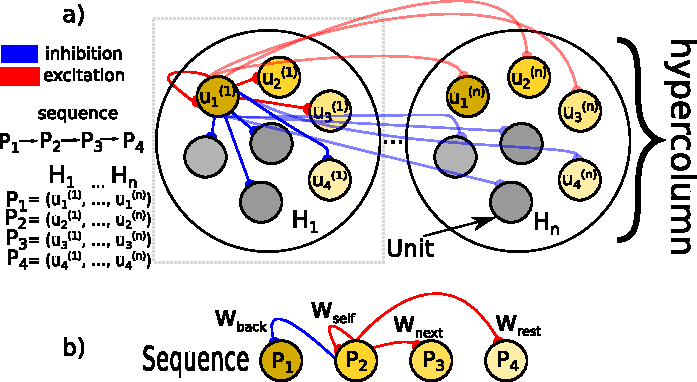
\includegraphics[scale=1.0]{diagram.pdf}
\caption{a) schematic of network structure. Units are organized into hypercolumns $H_1$, $\ldots$, $H_n$. At each point in time only one unit is active in each of the hypercolumns (small black circles). Patterns are defined as set of activated units across the hypercolumns. Pattern A, for example is the activation of unit 1 all the hypercolumns and can be represented by $A=(1, \ldots, 1)$. We depict stereotypical network connectivity by showing all the units that emanate from unit 1. The unit connects in excitatory fashion to the proximate units on the sequence (connections from 1 to 2 and 3) but it connects in an inhibitory fashion to both the units that are farther ahead on the sequence (1 to 4) and not in the sequence at all (1 to gray units). b) Depiction of important weights on sequence recall, the connections that emanate from pattern B and determine sequence dynamics are shown for subsequent characterization.}
\label{fig:networks_scheme}
\end{figure}


We model our units as collections of neurons with a population model equation \cite{wilson1972excitatory}. As described in equation \ref{eq:current} the current $s$ changes according to the base rate $\beta_i$ plus the total incoming current from the other units $ \sum_{j} w_{ij} o_j$. The binary activation variable $o_i$ represents unit activation and is related to the current through the WTA dynamics described in equation \ref{eq:non-linearity}. This  mechanism selects the unit receiving the maximum current at each hypercolumn and activates it. As a mechanism of pattern transition we implement a model of spike frequency adaptation through the adaptation current $a$ whose evolution is described by equation \ref{eq:adaptation}. Noise was introduced here with the white noise term $d\xi$. An extra current $I_i(t)$ to model the training signal and external influences on the model. For the sake of generality is important to stress that a our current based population model is mathematically equivalent to a rate based one as shown in \cite{miller2012mathematical}. 


\begin{align}
\tau_s \dfrac{ds_i}{dt} &= \beta_i + \sum_{j} w_{ij} o_j  - g_a a_i - s_i  + \sigma d\xi(t) + I_i(t) \label{eq:current} \\ o_i &=   \begin{cases}
       1,&  s_i = \underset{hypercolumn}{\max}(\mathbf{s}),\\
       0 ,& \text{otherwise}
    \end{cases} \label{eq:non-linearity} \\
\tau_a \dfrac{da_i}{dt} &= o_i - a_i \label{eq:adaptation} 
\end{align}


It has long been recognized that an assymetric connectivity in an attractor network produce to sequential dynamics \cite{amit1992modeling}. In that vein, we explain now how an asymmetric connectivity matrix coupled with the dynamics of our model brings about sequential dynamics. 
 
In figure \ref{fig:recall}a) we show a case of successful sequential recall in a system with the connectivity matrix depicted in \ref{fig:recall}d). Here we handcrafted the connectivity matrix to illustrate the unfolding of the dynamics which is as follows. First we cue the first pattern in the system with an input current for long enough so the pattern activates $o_i=1$. When a given pattern is active the adaptation current $a$ depicted in figure \ref{fig:recall}b) starts growing and as a consequence the self-excitatory current $s_i$ becomes smaller. At some point the self-excitatory current $s_i$ is going to become weaker than the feed-forward current $s_{i + 1}$  which the next pattern in the sequence is receiving. At that point the WTA dynamics of equation \ref{eq:non-linearity} kick-in and the next pattern becomes activated ($o_{i + 1}=1$) while the current one is extinguished by the same mechanism ($o_{i} =0$). These dynamics are self-sustained and the cycle repeats until the end of the sequence. We depict the profile of such transition in figure \ref{fig:recall}c). The total time that the pattern stays activated from its activation to its extinction is defined as the persistent time $T_{per}$ (also called dwelling time or switch time) and depends on the interplay between the connectivity matrix, the bias term and the adaptation as we now proceed to characterize.


\begin{figure}[H]
\centering
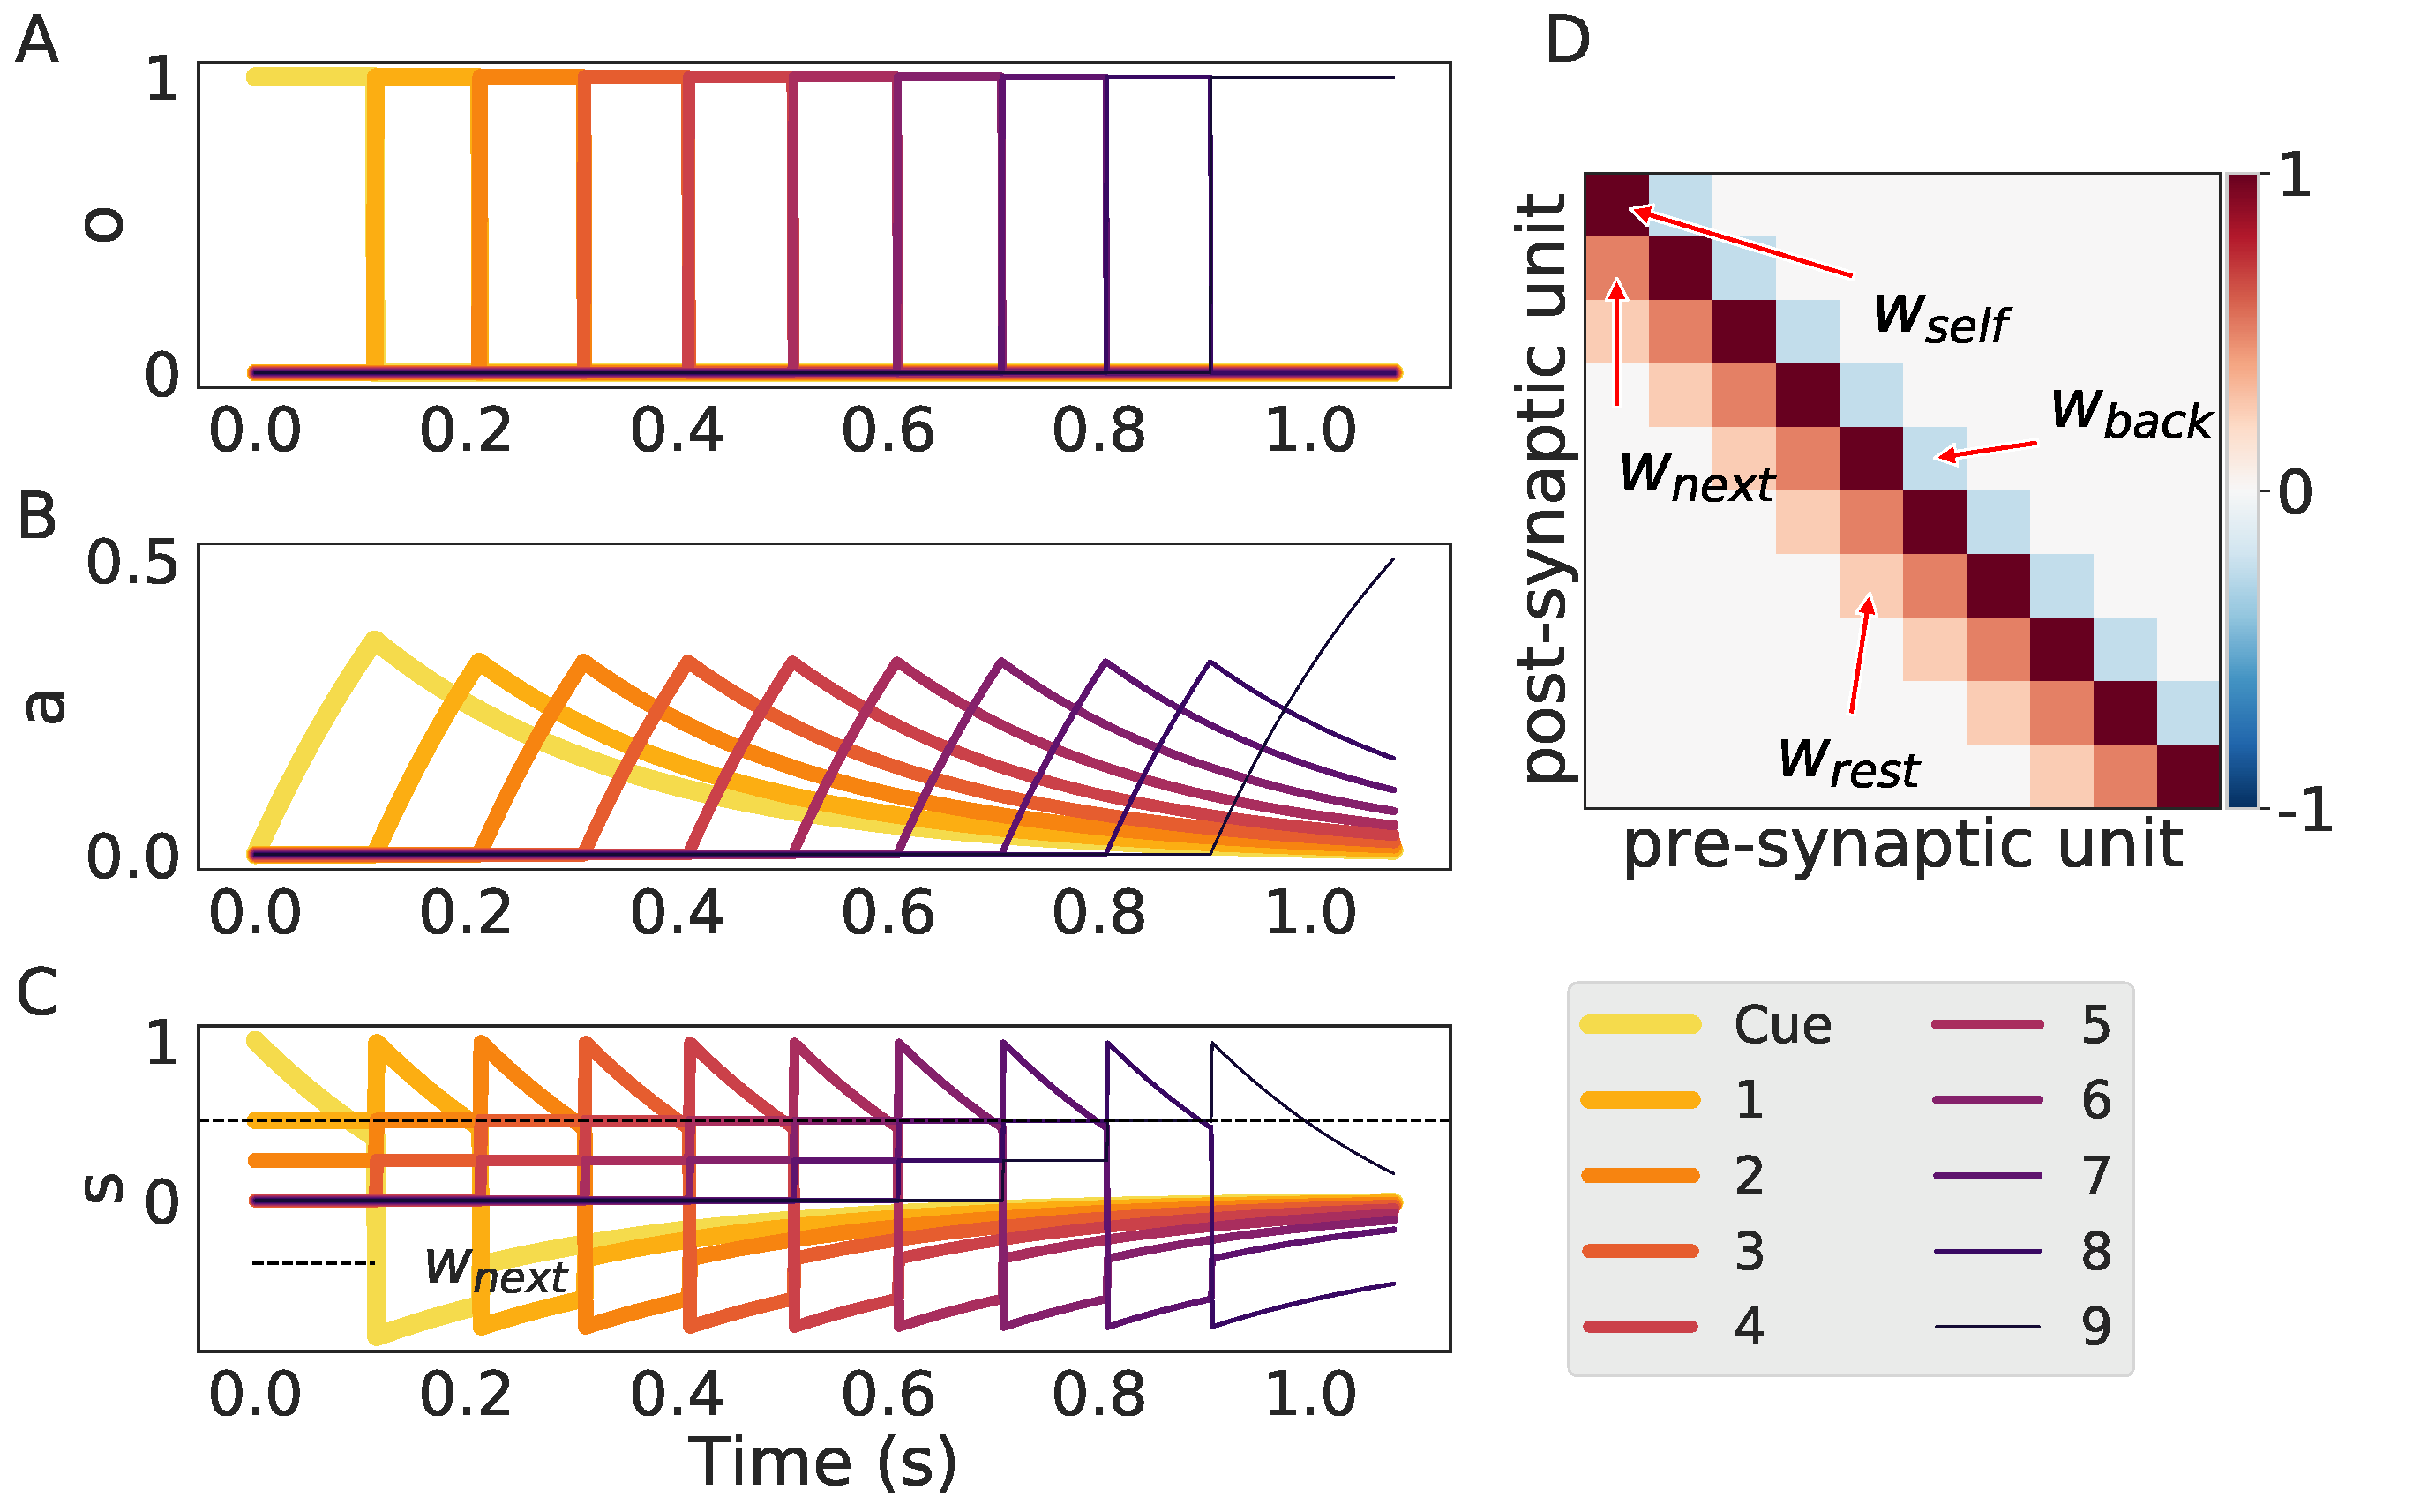
\includegraphics[scale=0.25]{simple_bcpnn_recall.pdf}
\caption{An instance of recall in the model. a) Unit activity starting with the cue. b) the time course of the adaptation current for each unit. c) total current $s$, note that this quantity crossing the value of $w_{next} o$ (depicted here with a dotted line) marks the transition point from one pattern to the next. d) The connectivity matrix where we have included pointers to the most important quantities $w_{self}$ for the self-excitatory weight, $w_{next}$ for the inhibitory connection to the next element, $w_{rest}$ for the biggest connection in the column after $w_{next}$ and finally $w_{back}$ for the connection to the last pattern that was active on the sequence.}
\label{fig:recall}
\end{figure}

\subsection{Persistent time}

Two important characteristics of sequence dynamics are the order in which the patterns are activated (the serial order) and the temporal structure of those activations (the temporal order) \cite{dominey2000neural}. 
In our model the serial order is determined by the differential connectivity between the current activated pattern and all the possible candidates. In general the next pattern activated will be the one for which the quantity $\Delta w_{next}  = w_{self} - w_{next}$ is smaller. The persistent time or temporal information of the sequence on the other hand is determined by the interplay between the connectivity of the network, the dyanmical parameters of the network and the external input to the network if it is available. We now proceed to characterize  this relationship analytically. From the deterministic trajectories (equation \ref{eq:deterministic_solution} in the appendix) we can find the point in time at which the currents from two subsequent units are equal: $s_i(t) = s_{i + 1}(t)$. Solving for t we determine the persistent time for each attractor determined with the expression in equation \ref{eq:persistent_times}.  

\begin{align}
T_{per} = \tau_a \log \left(\frac{1}{1 - B} \right) + \tau_a \log \left( \frac{                                                                                                                                                                                     1}{1 - \frac{\tau_s}{\tau_a}} \right) \label{eq:persistent_times}  \\ 
B = \frac{w_{self} - w_{next} + \beta_{self} - \beta_{next}+ I_{self} - I_{next}}{g_a} \\ 
B = \frac{\Delta w_{next} + \Delta \beta_{next} + \Delta I_{next}}{g_a} \label{eq:B_parameter}
\end{align}


The parameter B in equation \ref{eq:B_parameter} condenses the the information of the connectivity $w$, the bias terms $\beta$, tne adaptation strength $g_a$ and the external input $I$. From equation \ref{eq:persistent_times} we can infer that $T_{per}$ is defined only for $0 < B < 1$. This sets the conditions for how the weights, bias and external input interact with the adaptation parameters in order for the sequence to be learned and recalled. The straightforward interpretation for $B < 1$ is that the adaptation has to be strong enough to overcome the effects of the other currents. We summarize the effect of B on the $T_{per}$ in figure \ref{fig:per_time}. As illustrated in \ref{fig:per_time}a) $T_{per}$ is small for $B \sim 0$ and diverges to infinity as $B \sim 1$. This opens the door to think on $B$ as a unitless parameter whose natural interpretation is the inverse of transition speed as shown in the examples provided in figures \ref{fig:per_time}b) and \ref{fig:per_time}c).

We observe in figure \ref{fig:per_time}a) that system provides a logarithmic dynamical range for the values of $T_{per}$. This, while in theory, is infinite for perfect control of $B$ in practice has a lower bound determined by the time constant of the units $\tau_s \sim 10 \: ms$  (figure \ref{fig:min_time_encoding} in the appendix) and an upper bound imposed by our lack of precision in our ability to place the value of $B$ close to $1$.  We illustrate the relationship between the precision of $B$ and the maximum persistent time $T_{max}$ in figure \ref{fig:per_time}d). For a precision of $0.1$ the maximum persistent time attained with $T_{max} = 585 \:ms$ (marked with a red square in figure \ref{fig:per_time}d)) which can be double or halved by doing the same to the adaptation time constant $\tau_a$ in equation \ref{eq:persistent_times}. This already gives us a dynamical range of an order of magnitude (from $10$ ms to $1.0$ ms). Longer dynamical ranges can be achieved with higher precision in our control of $B$ as illustrated in figure \ref{fig:per_time}d). 

The idea that the serial order is controlled by the overall connectivity of the network while the temporal structure of the sequence is controlled by short term dynamics has been discussed before \cite{veliz2015networks}. In our model the temporal structure of the sequence can be controlled  by the adaptation dynamics. Choosing specific values of $g_a$ for different units allow us to control $T_{per}$ for every atractor in a precise way as we illustrate in figure \ref{fig:per_time}e). Differential temporal structure can also be attained by external control through the external current $I(t)$, this is align with the findings of temporal control in striato-cortical circuits \cite{murray2017learning}. 


\begin{figure}[H]
\centering
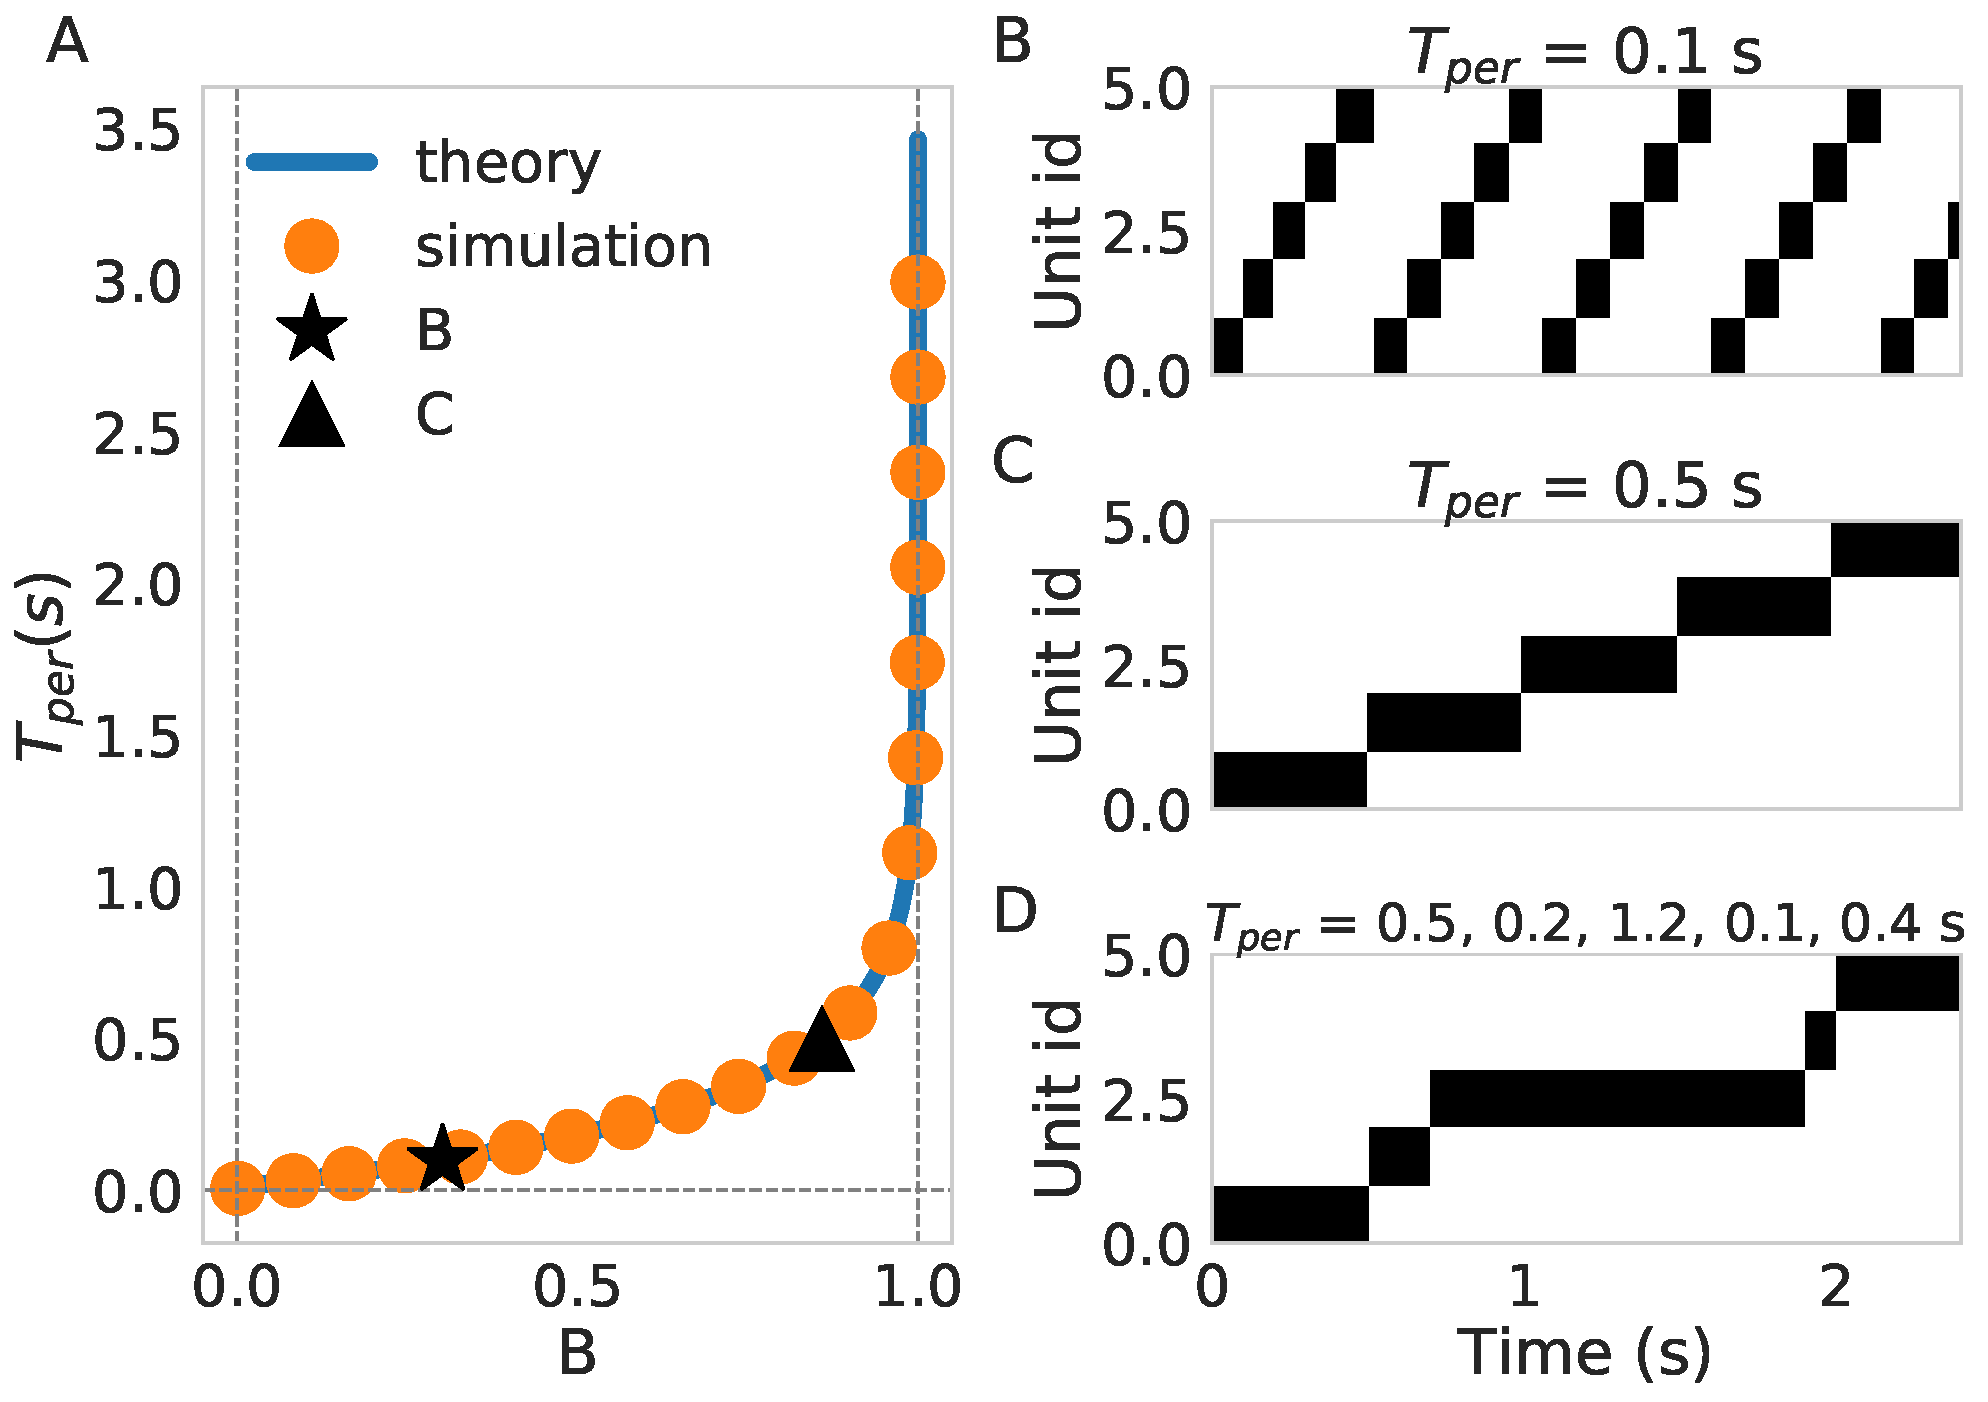
\includegraphics[scale=0.30]{persistent_times.pdf}
\caption{Systematic study of persistent time $T_{per}$. a) $T_{per}$ dependence on B. The blue solid line $T_{per_{theo}}$ represents the theoretical prediction described in equation \ref{eq:persistent_times} and the orange bullets $T_{per_{sim}}$ are the result of simulations. We show two examples of time encoding in b) and c). The first with $T_{per}=100 \: ms$ and the second with $T_{per}=500 \: ms$; both are also shown in a) marked with a start and a triangle respectively. d) relationship between the precision over B and $T_{max}$ the maximum attainable persistent time. We mark with a square $T_{max}=585 \:ms$  when we can get B to a tenth of 1.0. The shades represent the possible values obtained by varying $\tau_a$ between $0.5$ and $2$ of its usual value ($\tau_a = 250 \: ms$). e) example of variable encoding of attractor time with $T_{per}$ values of $500$, $200$, $1200$, $100$, and $400 $ ms respectively.}
\label{fig:per_time}
\end{figure}

\subsection{Learning}

So far we have shown that our model can support sequence learning and control the temporal structure of sequence recall through the adaptation dynamics. We now show that it if the network is subject to the right spatio-temporal input structure then associative hebbian learning is sufficient to induce a self-organizing process leading to the right asymmetric connectivity structure. As a model of associative learning and based on previous work we utilize here the BCPNN learning rule \cite{lansner1989one} in its incremental on-line version \cite{sandberg2002bayesian} with learning mediated through asymmetric time traces \cite{tully2016spike}. The version of the BCPNN learning rule presented here can be considered the simplest generalization to a continous setting of the discrete learning rule presented in  \cite{lansner1989one} (see the apendix). 

\begin{align}
\tau_{z_{post}} \dfrac{dz_i}{dt} &= o_i - z_i 
& \tau_{z_{pre}} \dfrac{d z_j}{dt} &= o_j - z_j \label{eq:z_traces} \\
t \dfrac{dp_i}{dt} &= z_i - p_i  
\qquad \quad t\dfrac{dp_{ij}}{dt} = z_i z_j - p_{ij}
&t\dfrac{dp_j}{dt} &= z_j - p_j    \label{eq:p_traces} \\
w_{ij} &= \log \left(\frac{p_{ij}}{p_i p_j} \right) & \beta_i &= \log(p_i) \label{eq:bcpnn} 
\end{align}

We now describe the learning equations. The two equations in \ref{eq:z_traces} are called the z-traces. Formally they are a low-passed filtered version of the activation units $o$ and they can be thought as variables that dynamically track the activation as shown in the top of figure \ref{fig:training_protocol} where we show the $z_{pre}$ trace for unit B and the $z_{post}$ for unit C. The equations \ref{eq:p_traces} implement an online and continous version of the average over the z-traces.  The idea of the BCPNN learning rule is to create excitatory connections between units that were activate together in the training process and therefore belong to the same pattern and create negative connections among those who did not. To achieve this the $w_{ij}$ term in equation \ref{eq:bcpnn} weights the joint probability $p_{ij}$ against the independent probability of activation $p_i p_j$; if the former is bigger than the latter the connection is excitatory if this is not the case then the connection is inhibitory. In the discrete version of the BCPNN the probabilities are estimated from the activations $o$ only. This implies that patterns that are not active at the same time are not associated to each other making the temporal binding required for sequence learning unfeasible. Here however, we estimate the probabilities from the z-traces which implies that the contiguous temporal adjacency of patterns in a sequence leads to co-activations as illustrated in the red area of the figure \ref{fig:training_protocol}. The result is that training sequences results in the assymmetric connectivities with feed-foward connections that are needed to sustain sequential recall of attractors, an example of such training process is shown in figure \ref{fig:recall_example}c).  In order to deal with the possibility of arguments with value 0 in the logarithmic we have set a lower bound of $\epsilon = 10^-7$ for the p-traces. This sets a lower bound on the value of the weights at $-7$, we explain the rationality of such choice in the appendix. 

%\begin{align}
%\tau_{z_{post}} \dfrac{d\underset{post}{z_i}}{dt} &= o_i - \underset{post}{z_i} 
%& \tau_{z_{pre}} \dfrac{d\underset{pre}{z_i}}{dt} &= o_i - \underset{pre}{z_i} \label{eq:z_traces} \\
%t \dfrac{dp_i}{dt} &= \underset{pre}{z_i} - p_i  
%\qquad \quad t\dfrac{dp_{ij}}{dt} = z_i z_j - p_{ij}
%&t\dfrac{dp_i}{dt} &= \underset{pre}{z_i} - p_i    \label{eq:p_traces} \\
%w_{ij} &= \log(\frac{p_{ij}}{\underset{pre}{p_i} \quad\underset{post}{ p_j}}) & \beta_i &= \log(p_i) \label{eq:bcpnn} 
%\end{align}
 

\begin{figure}[H]
\centering
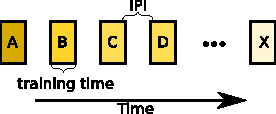
\includegraphics[scale=0.30]{protocol.pdf}
\caption{Top) learning by traces. The system weights the intersection of two traces (co-activation) against the base activation rate of each unit to determine the magnitude of the weight between two units. Note that the two z-traces are governed by different time constants. In this case the time constant of the $z_{pre}$ traces is far slower than the one from $z_{post}$. Bottom) the training protocol. We show here the basic scheme of the training protocol used in a system where pattern A, B, C, and D are learned in sequence.}
\label{fig:training_protocol}
\end{figure}

The training protocol shown in figure \ref{fig:training_protocol} is a model of the temporal nature of the input and can be characterized by two quantities. First we have the time that the network is exposed to pattern (this is implemented by units being clamped through $I$ in equation \ref{eq:current}), we call this the training time. Second, we have the time between the presentation of two patterns which we call the inter-pulse-interval (IPI). Note that while in generality neither the training time nor the IPI need not to be equal for each pattern, in the following and as a first approximation we characterize an homogeneous training protocol where both the training time and the IPI are equal for each pattern.

An example of a connectivity matrix resulting from training is show in figure \ref{fig:recall_example}b). Is notable that the connectivity matrix shows the desired asymmetric structure. We also show the recall process at the unit and the pattern level in a) and b) respectively. Finally to show how the the parameters of the training protocol affect the connectivity matrix we show in d) how the connectivity profile between a unit and all the others changes depending on the training time parameter. That is, in d) we trained the network for different training times and provided the connectivity profile for each of the outcomes. The structure of the sequence coupled with the asymmetric time constant of the z-filters results in the assymmetry between the backward and forward connections illustrated here. Finally for longer training times (lighter traces) the feed-forward connection decay faster due to the fact that two pattern activation are farther away from each other.


\begin{figure}[H]
\centering
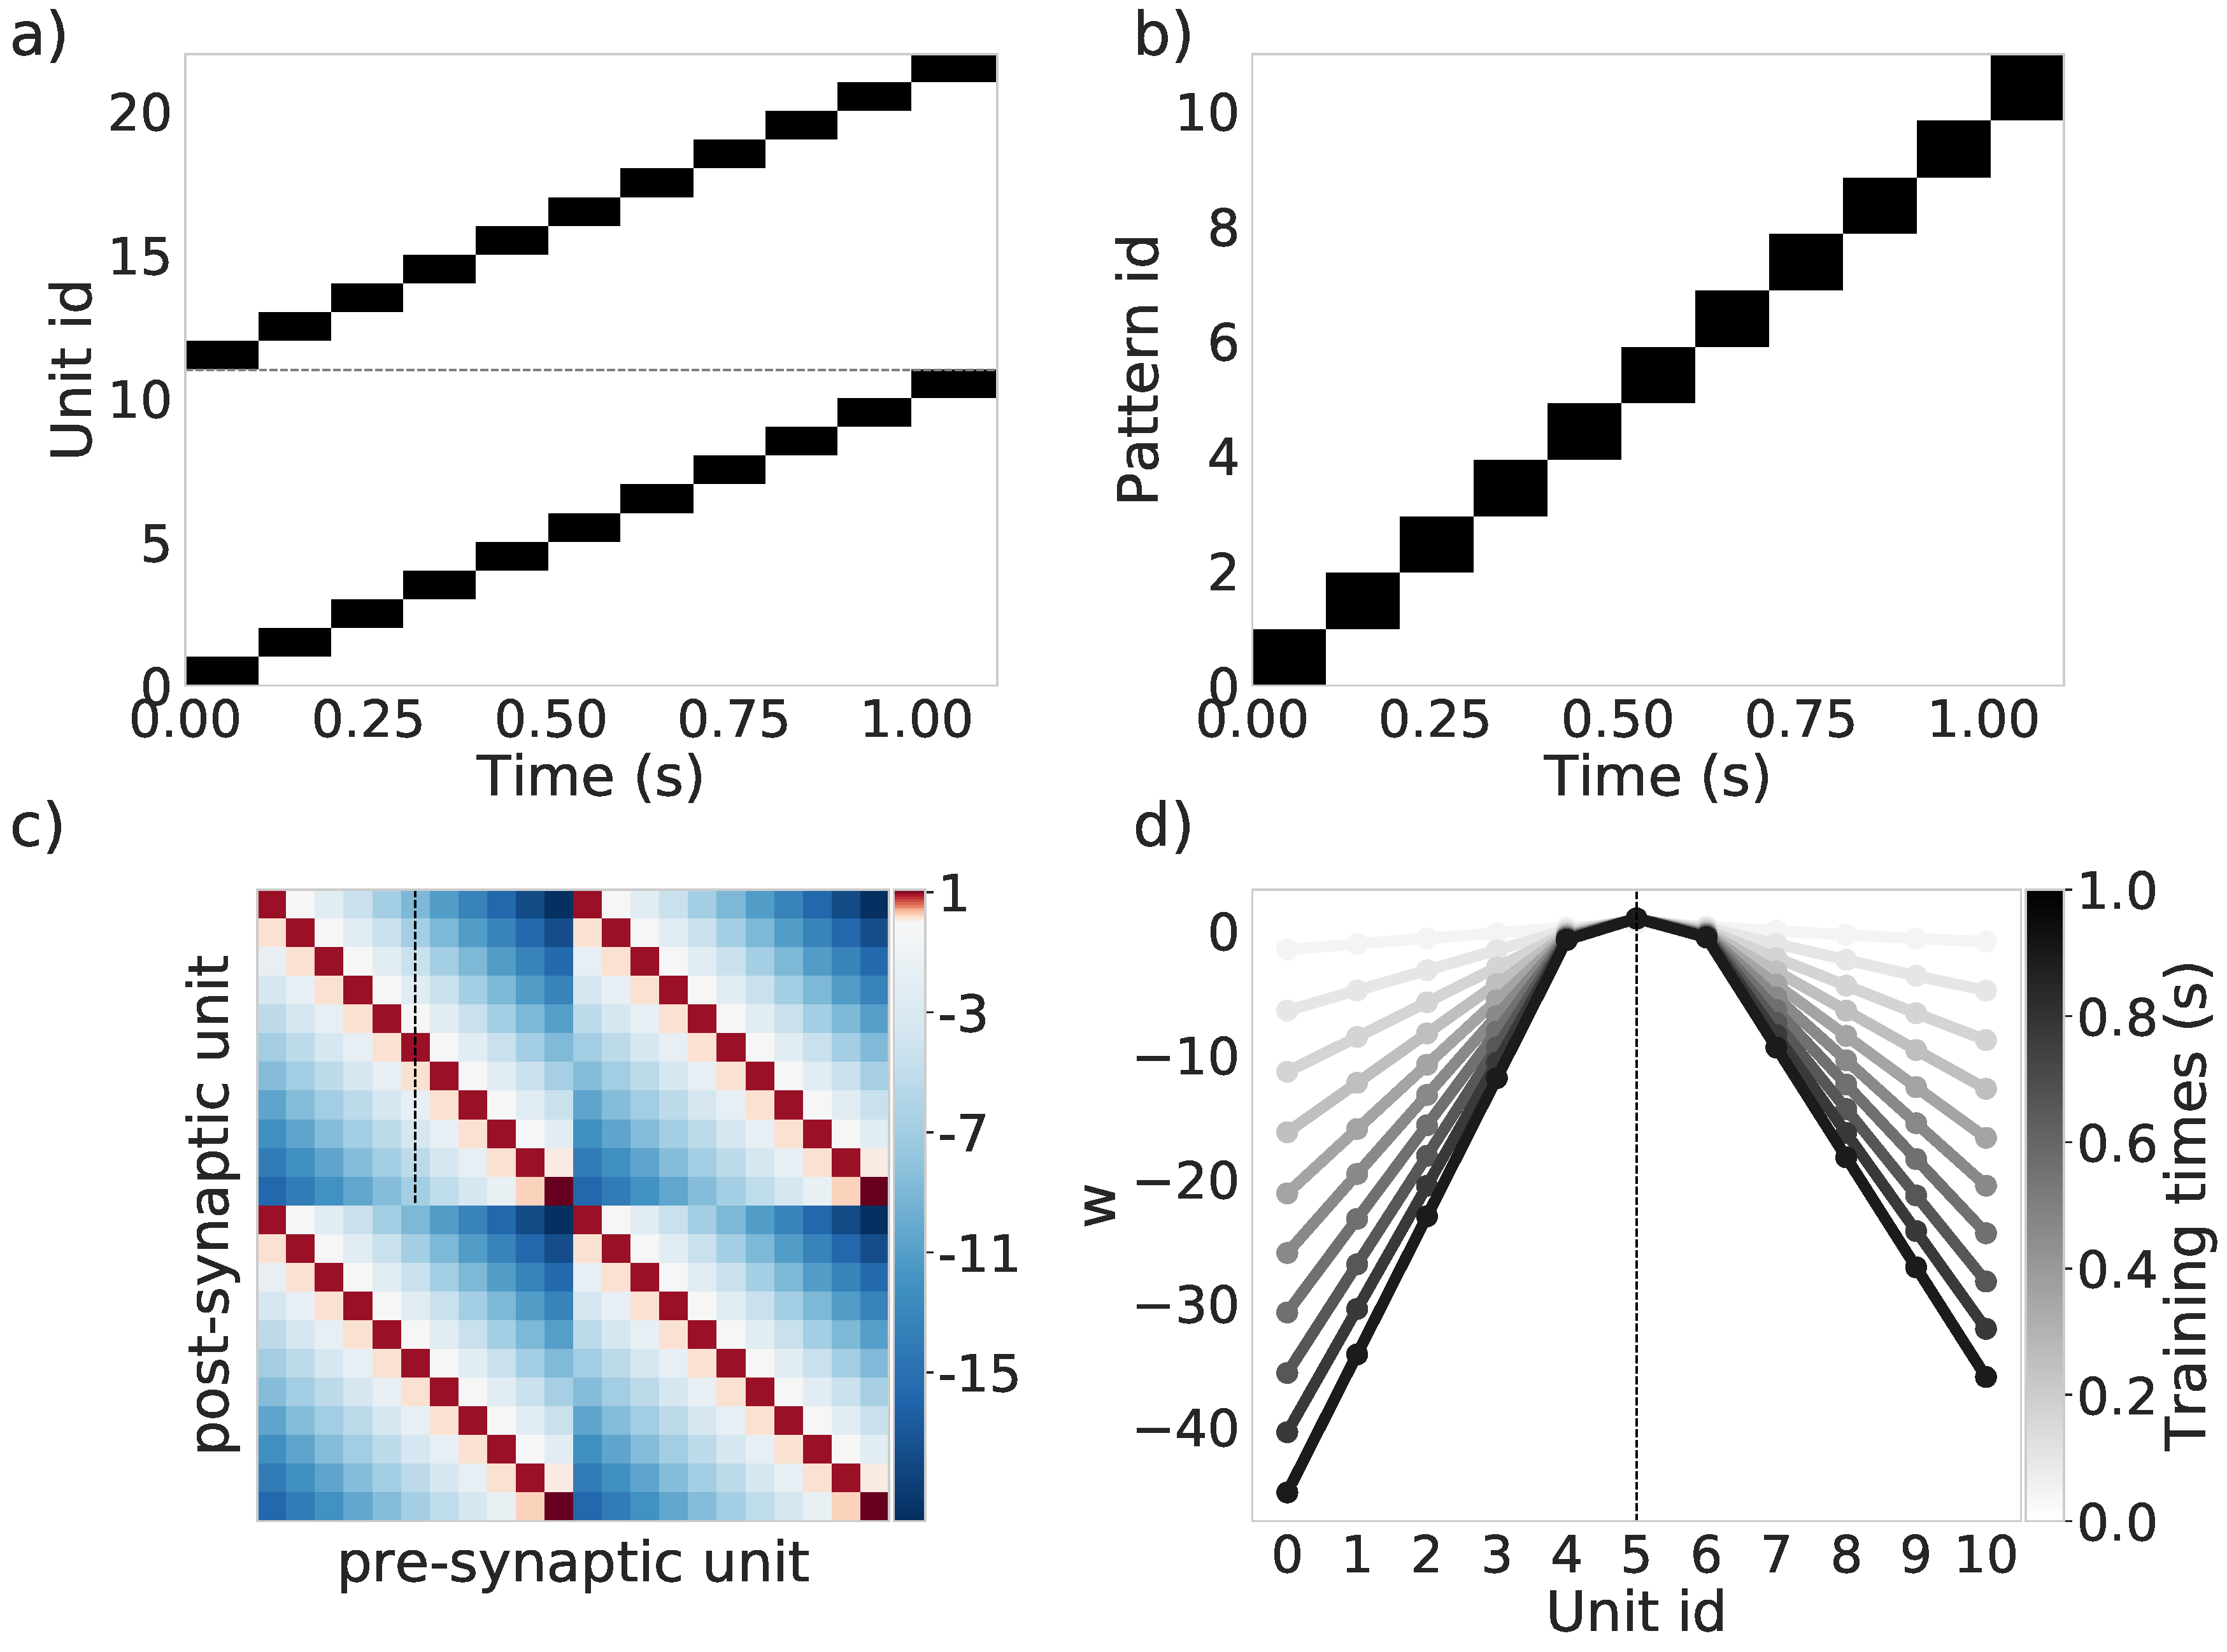
\includegraphics[scale=0.20]{recall_example.pdf}
\caption{An example of recall with 10 minicolumns and 2 hypercolumns, $\tau_{z_{pre}} = 25 \: ms$, $\tau_{z_{post}}=5 \: ms$, training times $=100 \: ms$ and $IPI = \: 0 $. a) recall phase in a system with learned connectivity. The division by hypercolumns is marked with a horizontal dashed line b) cosine similarity between the instant activity of the network and the stored pattern at every point in time. c) The connectivity matrix for this particular example, note the modular organization of the network.  d) connectivity profile for a variety of training times from $0$ to $500$ ms). Darker lines represent shorter training times. Note the asymmetry between the forward and the backward weights. The profile corresponds to the connections emanating from unit 5 towards all the units in the red dashed line in c).}
\label{fig:recall_example}
\end{figure}

%With a homogeneous training protocol $\Delta \beta_{next}=0$ and in in systems without external input $\Delta I_{next} = 0$ therefore we have that $B$ and in consequence $T_{per}$ only depend on $\Delta w_{next} = w_{self} - w_{next}$ which is indicated on the inset of figure \ref{fig:training}d)

We characterize the learning systematically in figure \ref{fig:training}.  In the following explanation everything that we say about $w_{next}$ can be applied to $w_{back}$ as they are generated with the same process but with flipped time constants on their filters. In figure \ref{fig:training} a) we observe that as the training time increases the value of $w_{self}$ quickly stabilizes but the value of $w_{next}$ becomes smaller progressively. This can be explained by the fact that while the ratio between self co-activation and the total training time remains more or less constant (stabilizing $w_{self}$) the co-activation between units becomes a smaller portion of the whole training protocol (making $w_{next}$ smaller). The consequence of this can be reflected in the figure \ref{fig:training}d) where we see that $T_{per}$ rate of growth becomes constant with bigger training times giving a logarithmic encoding of time. In figure \ref{fig:training}b) is shown that $w_{self}$ keeps increasing while $w_{next}$ is decreasing with longer IPIs. The reason for this is that IPIs bring about an overall longer training protocol which makes the self co-activation more meaningful and $w_{self}$ bigger but at the same time a longer IPI makes the co-activation between the units smaller as their activations are father from each other in time which leads to a decrease in $w_{next}$. As a consequence $T_{per}$ increases faster with longer IPIs as both $w_{self}$ and $w_{next}$ pull away from each other this effect is shown in figure \ref{fig:training}e). The effect of the z-filters time constant $\tau_z$ is summarized in the figure \ref{fig:training}c). The results can be explained by interpreting the effect of increasing $\tau_{z_{pre}}$ as diffusing the activation in time making co-activations less meaningful overall. This is reflected by the fact that $w_{self}$  and $w_{next}$ are pulled closer to each other meaning that the system distinguishes less and less between one pattern and the next. Note here that the point at which $\tau_{z_{pre}}$ becomes bigger than $\tau_{z_{post}}$ (marked with a dashed red line) coincides with $w_{next}$ becoming bigger than $w_{back}$ as we should expect. We can observe also that  $\Delta w_{next}$ becomes almost zero for big values of $\tau_{z_{pre}}$ which is reflected on figure \ref{fig:training}f) as smaller and smaller values for $T_{persistent}$. 


\begin{figure}[H]
\centering
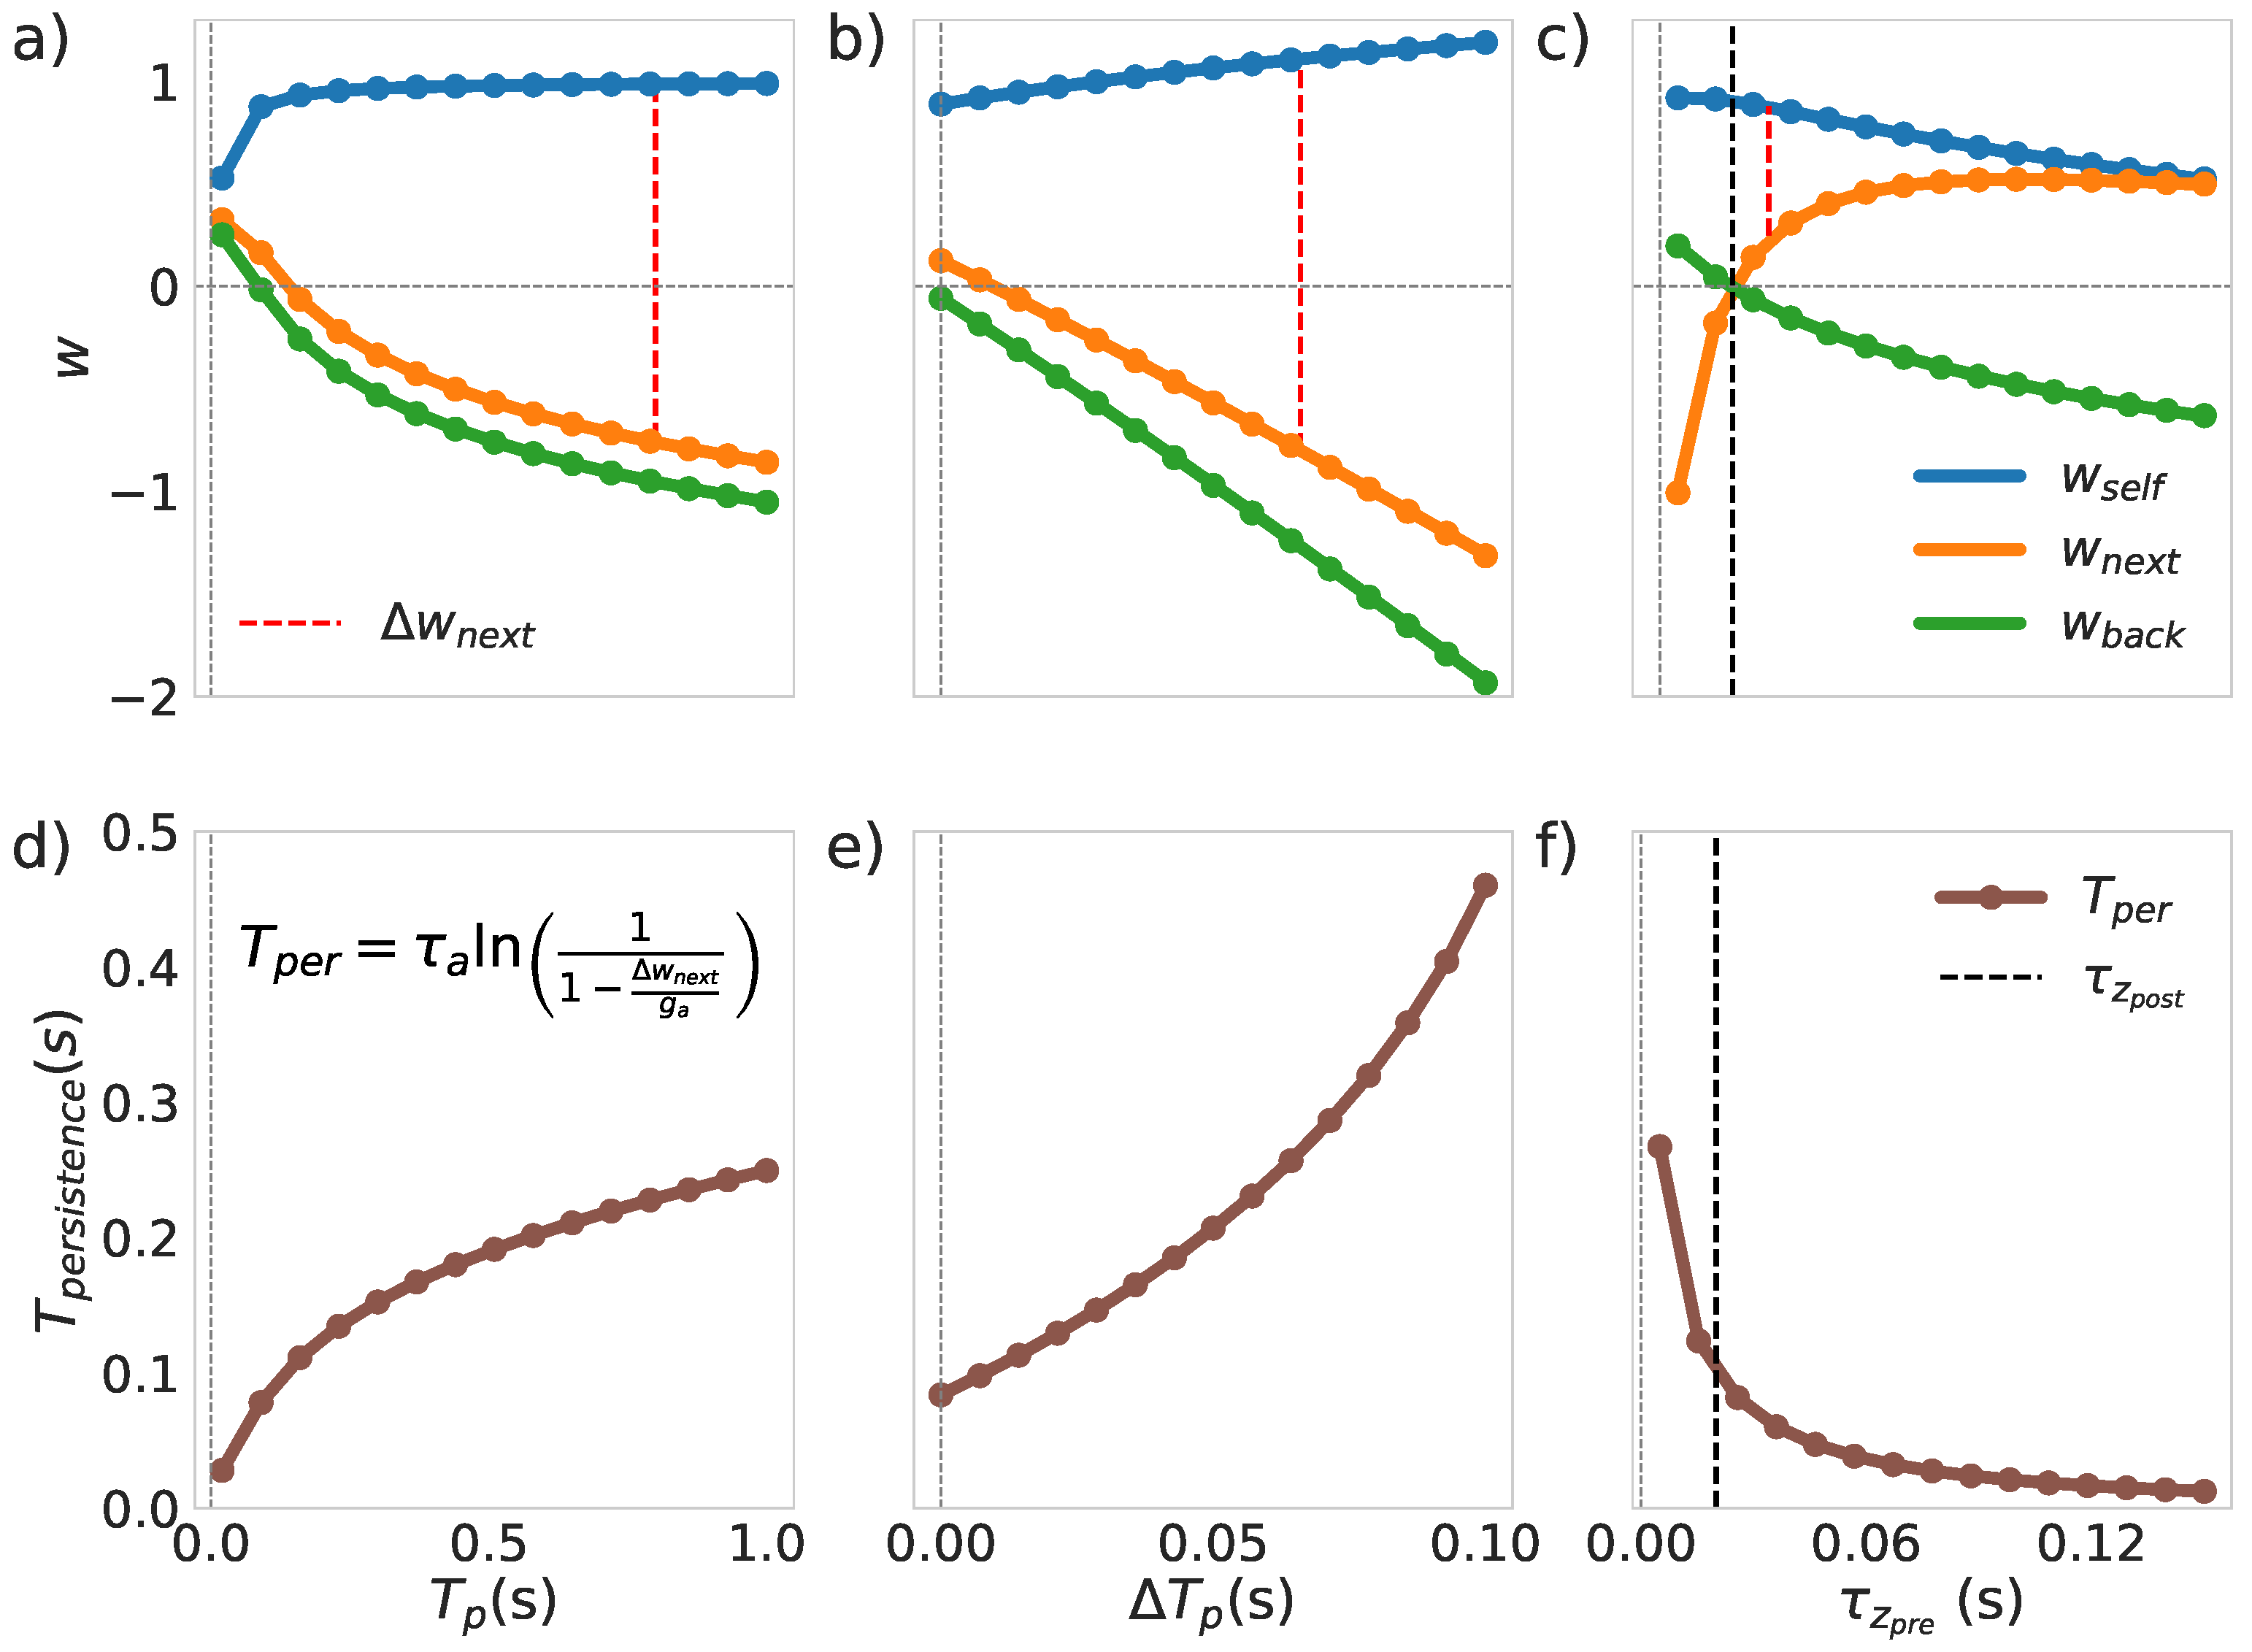
\includegraphics[scale=0.20]{training.pdf}
\caption{Characterization of the connectivity as a function of the training protocol. Here we show how the $w_{self}$, $w_{next}$, $w_{back}$ depend on the training protocol parameters. We also show the effects of training on the persistent time of the attractors $T_{per}$. The equation on the inset in d) relates $T_{per}$ to $\Delta w_{next} = w_{self} - w_{next}$ which we show as a dashed red line on the top figure. When the parameters themselves are not subjected to variation their values are: training time = $100 \: ms$, IPI $= 0 \: ms$, $\tau_{z_{pre}}  = 25 \: ms$, $\tau_{z_{post}}= \: 20 ms$ for all the units. a, b, and c show how the weights depend on the training parameters training times, IPI and $\tau_{z_{pre}}$ respectively whereas d, e and f show how this affects the $T_{per}$ or the encoding of time. }
\label{fig:training}
\end{figure}


The spatio-temporal structure of the input can change the recall phase from one where the pattern are binded in time in time in a sequence (sequence regime) to one where the patterns are learned independently (free attractor regime). We characterize. The mechanism that bridges the temporal gap (IPI) between the patterns is the time window given by the z-traces time constant $\tau_{z_{pre}}$. It is not surprising then that if we make the gap that the window has to bridge large enough (IPI large) or the bridging mechanisms less efficient through a smaller value $\tau_{z_{pre}}$ the sequential nature of the input will be lost in the learning. We characterize the parameter regime for this two dynamical schemes in figure \ref{fig:attractors}.  


\begin{figure}[H]
\centering
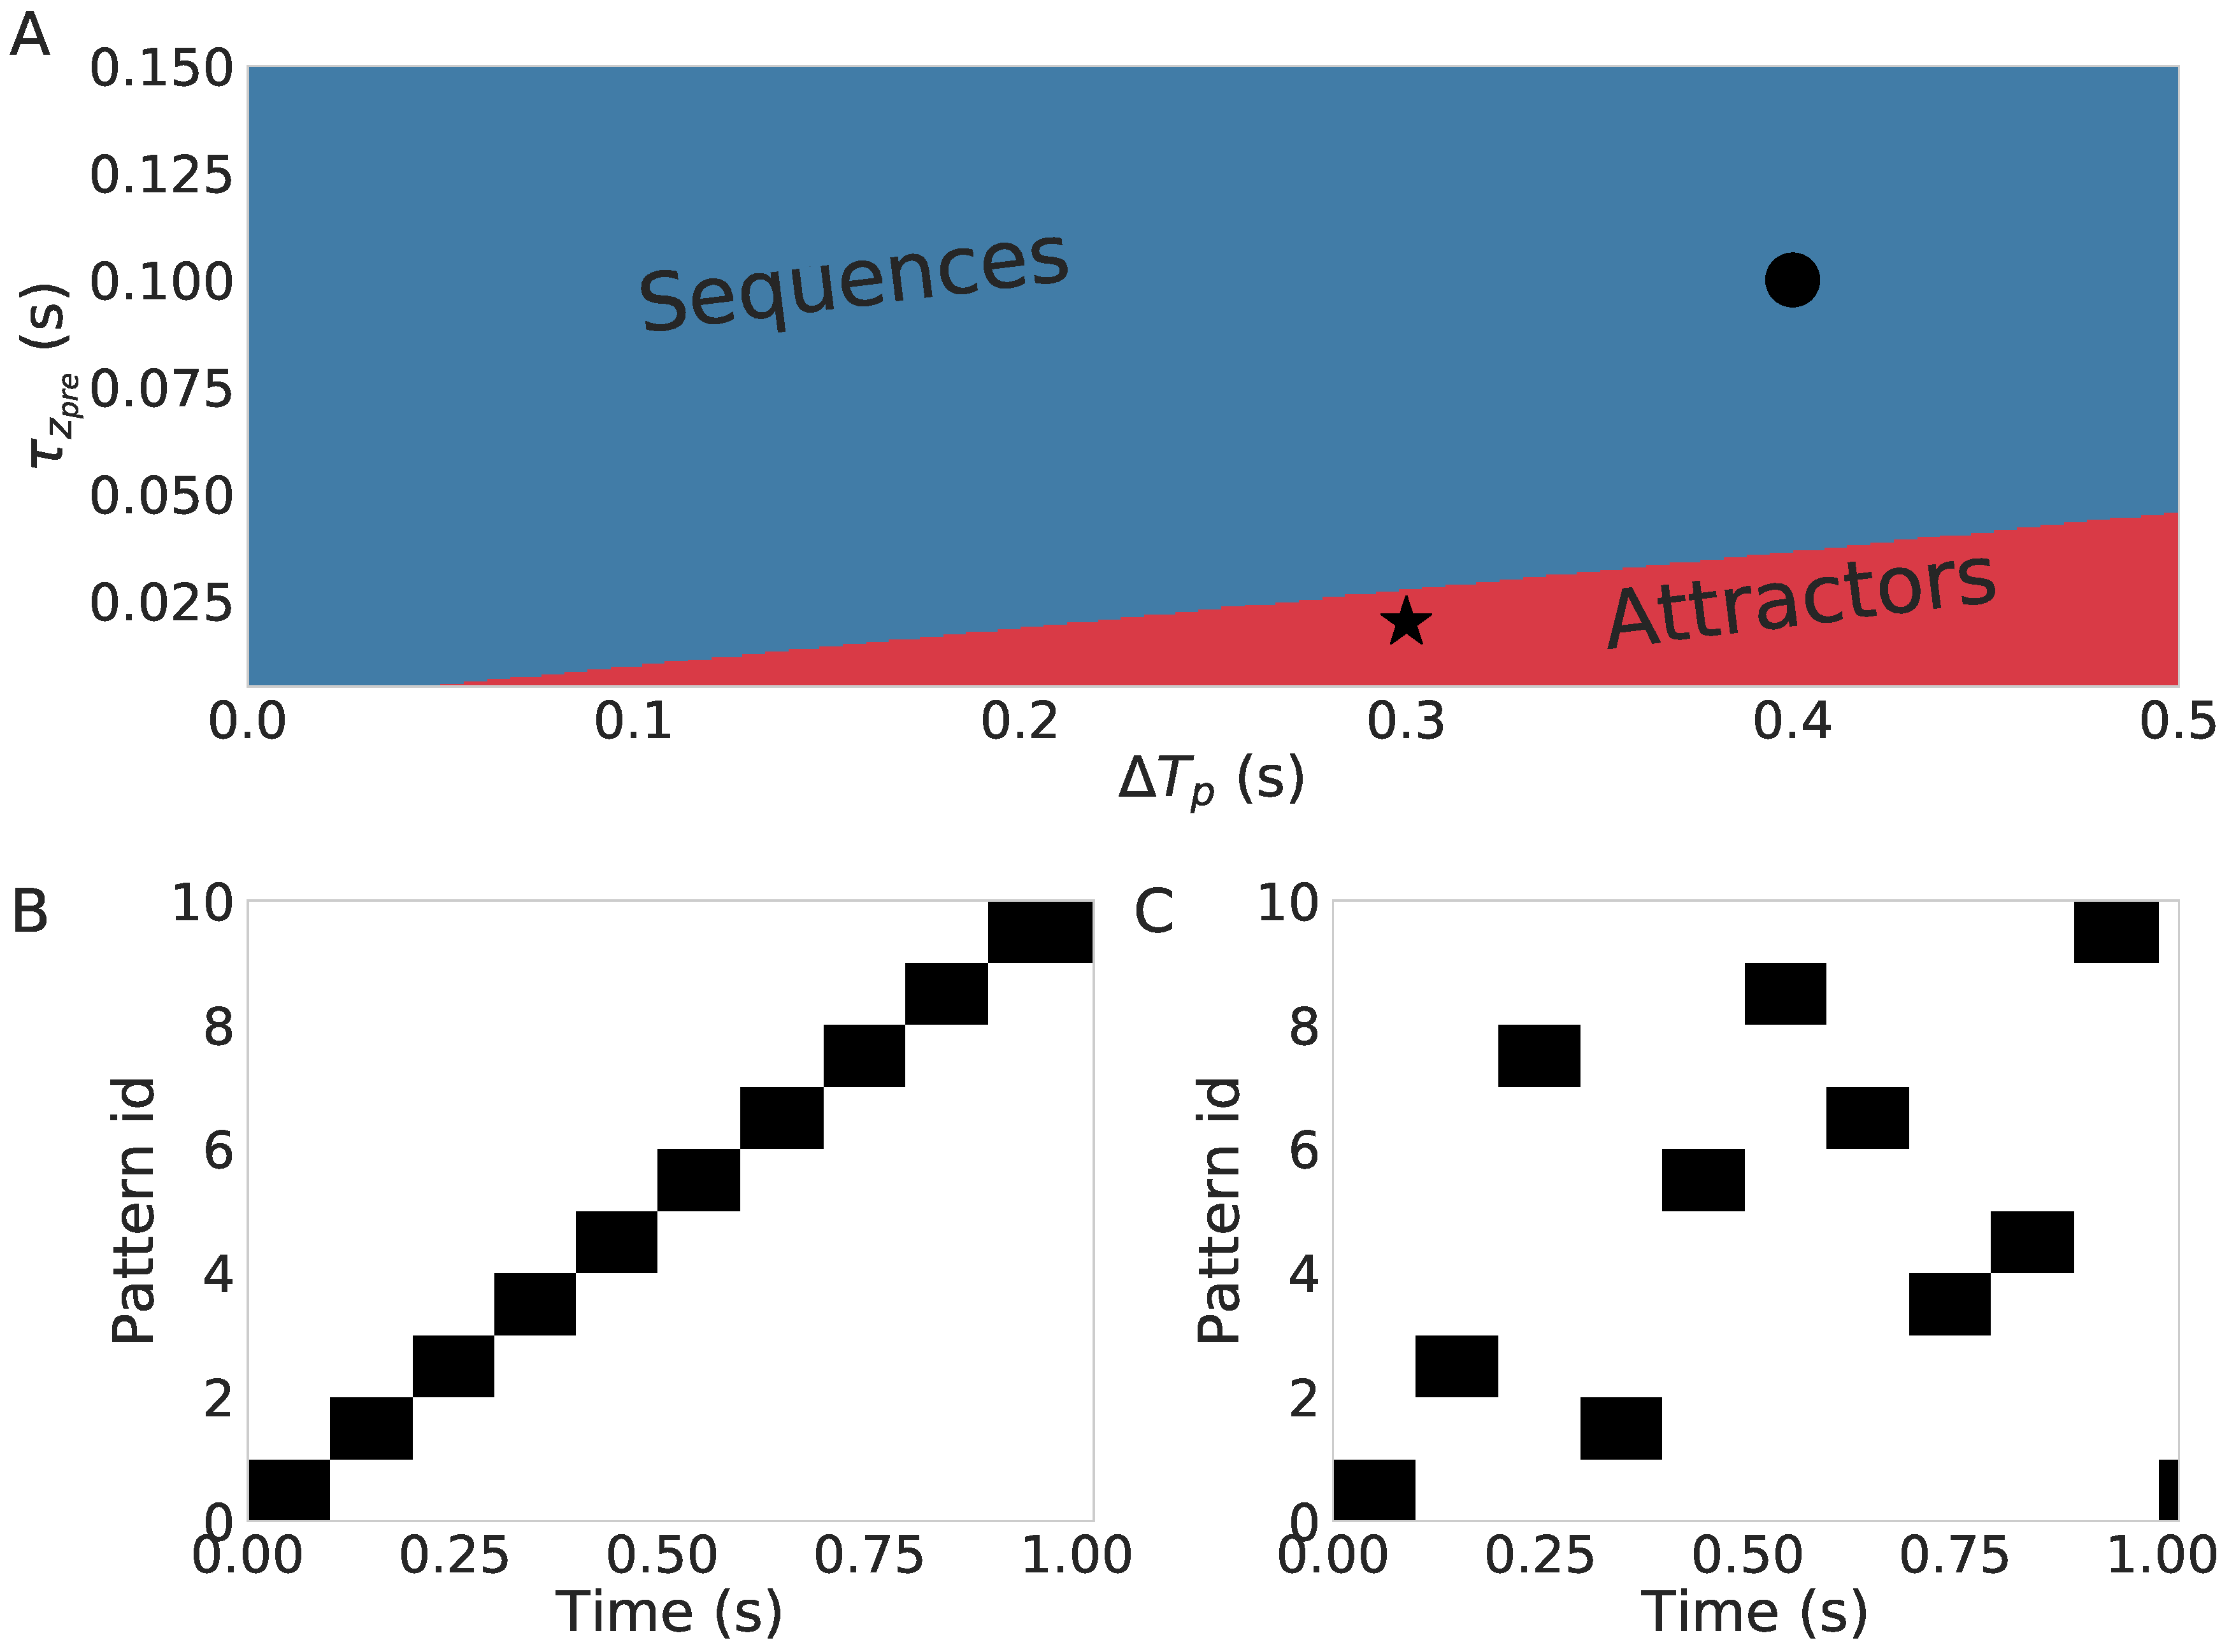
\includegraphics[scale=0.20]{attractor_vs_sequence.pdf}
\caption{Transition from the sequence regime to the free attractor regime a) we characterize how the interplay between the structure of the input IPI and the parameters of the network $\tau_{z_{pre}}$ brings about two different recall arrangements . b) we show the dynamic behavior (sequence regime) of the network at the point marked with a black circle in a). c) we show the dynamic behavior (free attractor mode) of the point marked with a star in a).}
\label{fig:attractors}
\end{figure}

\subsection{Noise}

We now test whether and how our system is robust to noise. In order to so we controlled the level of noise with the parameter $\sigma$ in equation \ref{eq:current}. Current noise in the evolution of the system creates stochastic trajectories which we illustrate in figure \ref{fig:noise_scheme} a). In a noisy environment the network make the transition to the next pattern faster that they would have done in the deterministic case. This is phenomena is illustrated clearly in the red and purple lines patterns where the noisy trajectories make the transition far sooner compared to their deterministic counterparts (thin transparent lines compared to solid lines). This means that a pattern subjected to noise will see its value of $T_{per}$ decreased by this effect. We characterized this trend systematically in figure \ref{fig:noise_scheme}b) where we subjected networks with different values of $T_{per}$ to different levels of noise resulting in the average value of $T_{per}$ decaying systematically with increasing values of $\sigma$. We may as well wonder whether encoding for shorter $T_{per}$ would have an effect on the overall recall capabilities of the network. In figure \ref{fig:noise_scheme}c) we show that the success rate vs noise profile does not show strong dependency on the encoded persistent time.  


\begin{figure}[H]
\centering
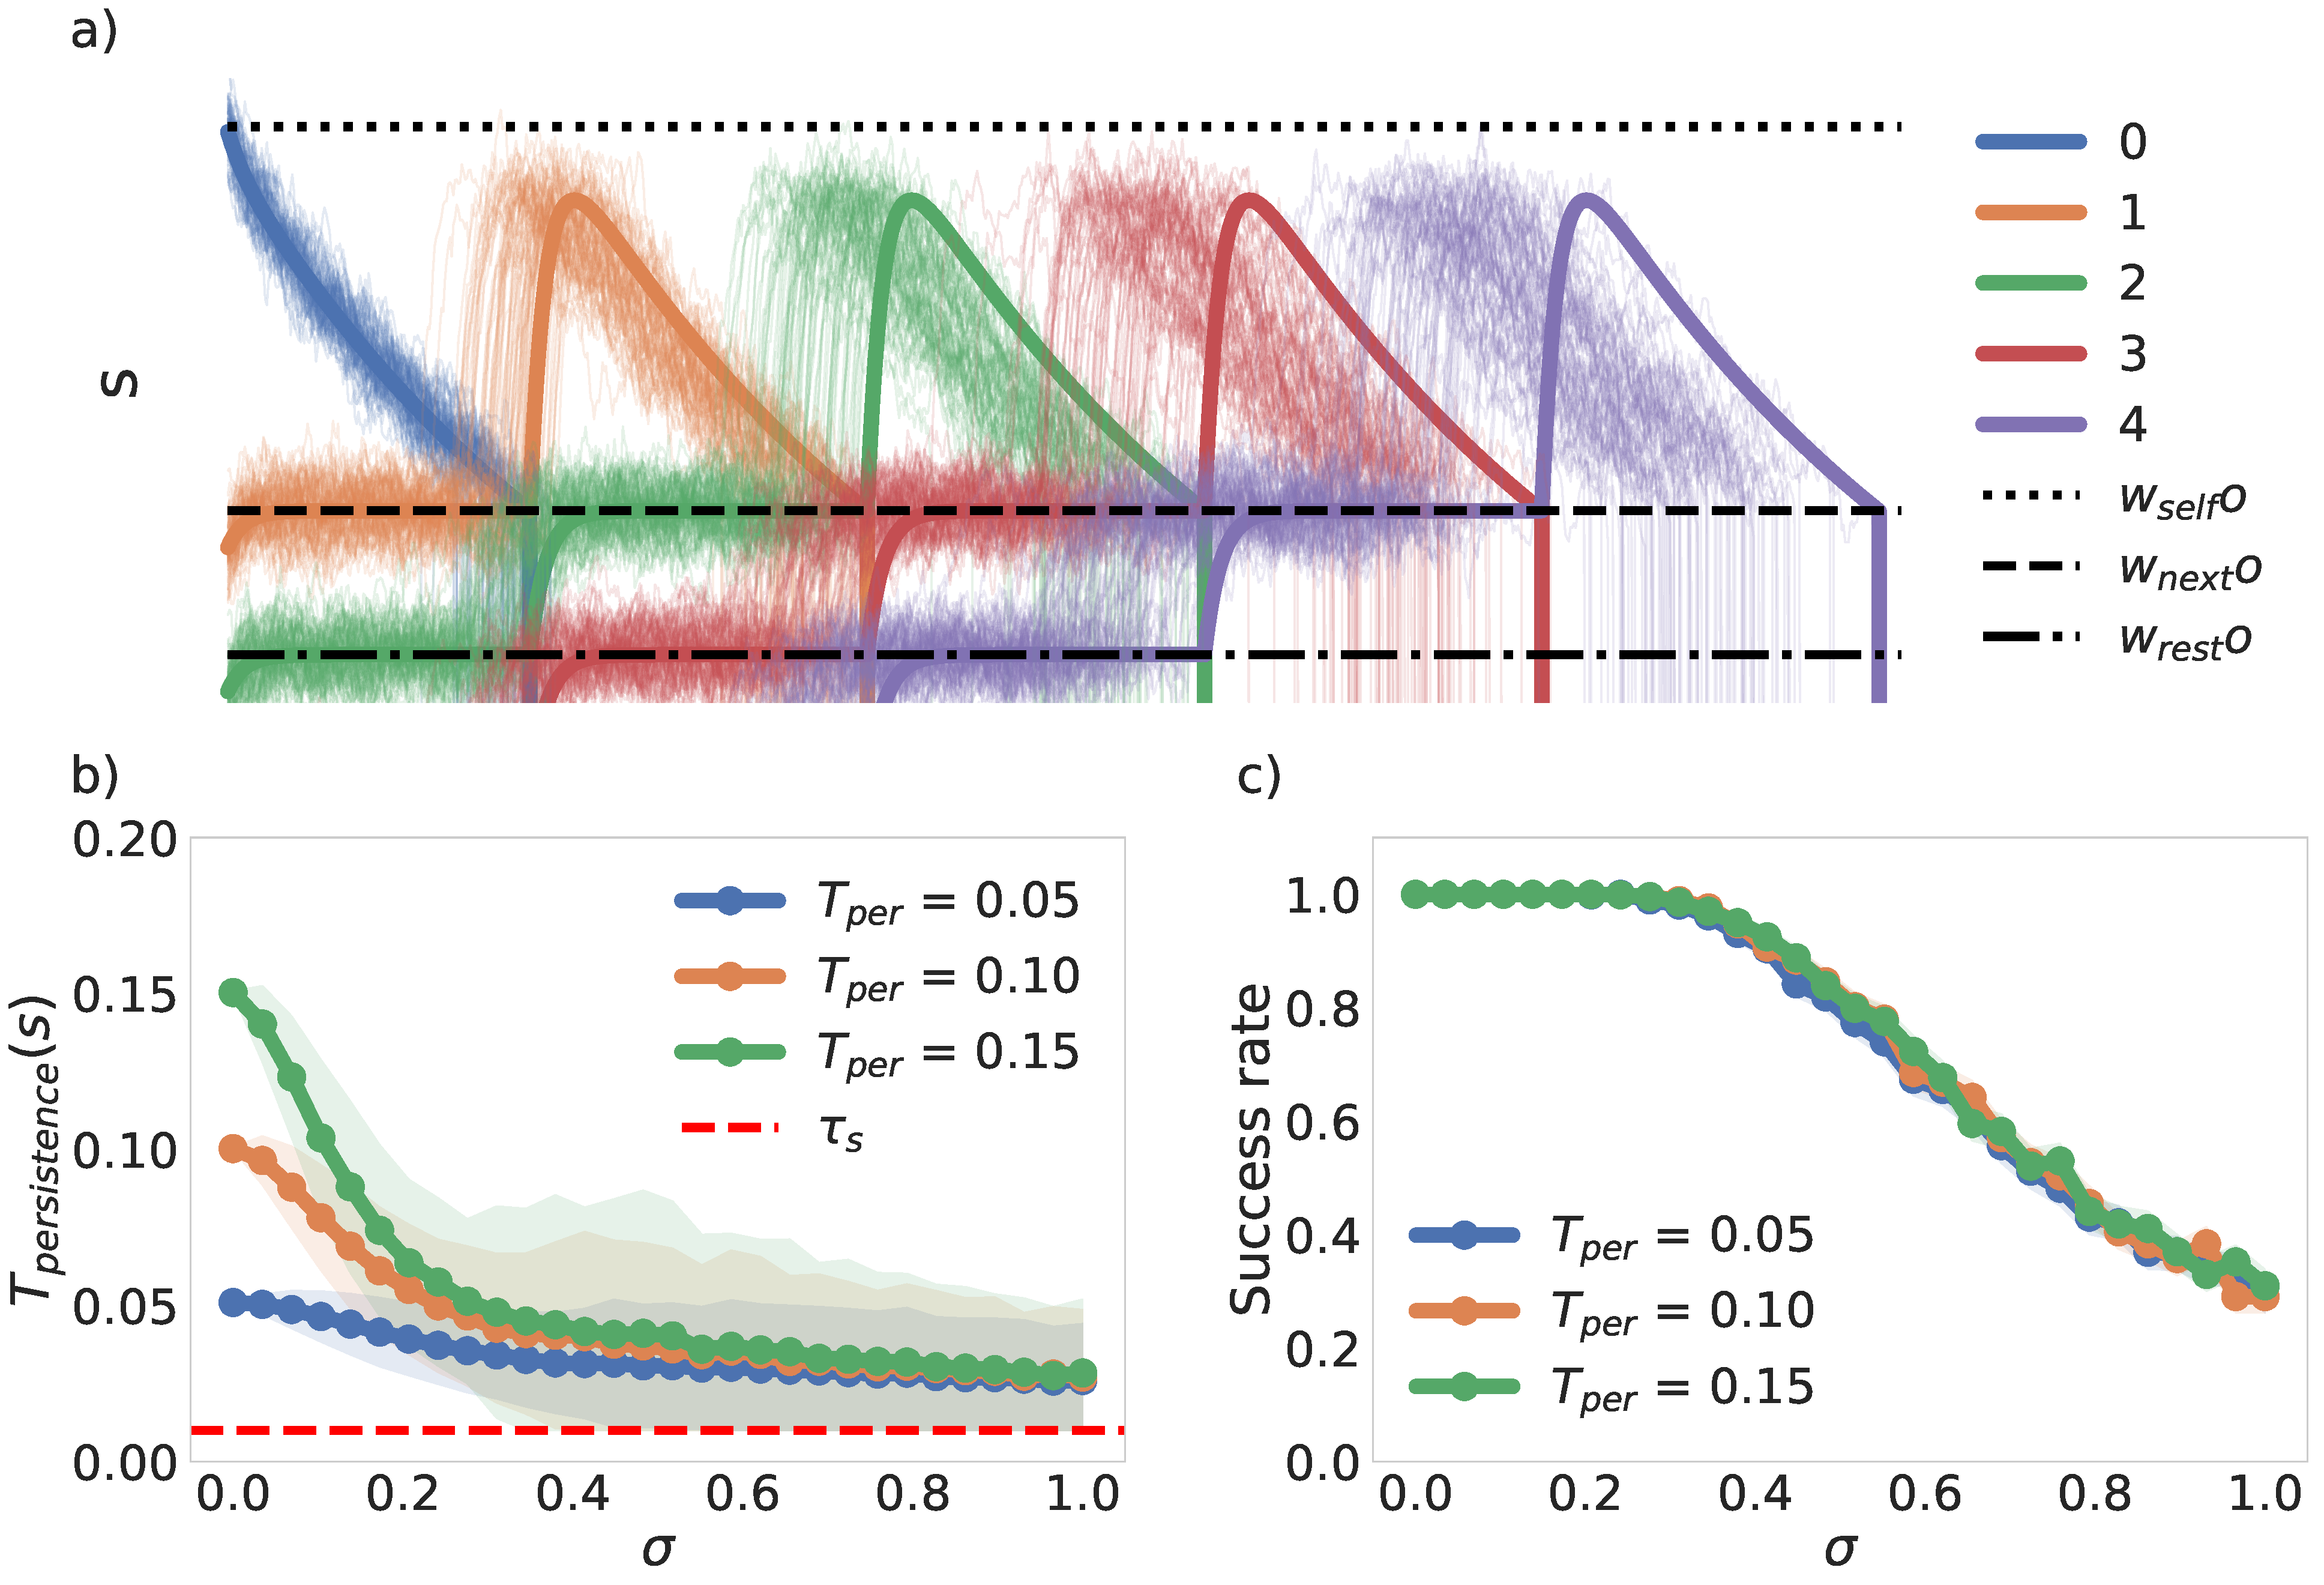
\includegraphics[scale=0.17]{noise_diagram.pdf}
\caption{Effects of noise in current trajectories and persistent time. a) an example of current trajectories subjected to noise. The solid lines indicate the deterministic trajectories the system would follow in the zero noise case. In dotted, jagged and dashed lines we depict the important landmarks of connectivity $w_{self}$, $w_{next}$ and $w_{rest}$ respectively. b)  average $T_{per}$ dependence on noise for networks encoded to have different $T_{per}$. c) success rate vs noise profile dependence on  $T_{per}$. We ran $1000$ simulations of recall and counted how many were successfully recalled as a function of $\sigma$. }
\label{fig:noise_scheme}
\end{figure}

Next we systematically characterized the sensitivity of the system to noise as a function of the training parameters of the network. We proceeded by calculating the value of $\sigma$ at which the success rate becomes less than $\frac{1}{2}$. We illustrate the nature of such values in figure \ref{fig:noise_sensitivity}a), note that the bigger $\sigma_{50}$ is the less sensitive the system is to noise and vice versa. In the figure \ref{fig:noise_scheme}b) we show how $\sigma_{50}$ changes as we change the training time, we can see that the system becomes less sensitivity to noise the longer it is trained. This can be explained by the fact that training for longer increases the overall distances between the weights as shown in figure \ref{fig:training}a). We can see the same effect by increasing the IPI in figure \ref{fig:noise_sensitivity}c) where the separation of weights produced by longer $IPI$ leads to the same outcome. The opposite effect is observed in figure \ref{fig:noise_sensitivity}d) where the system becomes more sensitive with longer $\tau_{z_{pre}}$. We can appeal again to the structure of the weights in figure \ref{fig:training}c) to explain this results as an outcome of the weights becoming less differentiated among themselves. 

We also have two noise effects that are not related to the connectivity effects. First in \ref{fig:noise_sensitivity}e) we show that sequence recall becomes more sensitive to noise the longer a sequence is. This can be explained by thinking on every link on the chain as a possible point of failure in itself. Naturally, adding more links to the chain makes it more likely for the sequence to fail at some point. Finally, in figure \ref{fig:noise_sensitivity}f) we show that there is a scaling effect with the number of hypercolumns. We can explain this effect by the creation of more robust representations where if a wrong transition occurs at a unit of some pattern the attractor effect of the remaining units of the pattern will correct for the local mistake and allow the sequence to be recalled successfully.

\begin{figure}[H]
\centering
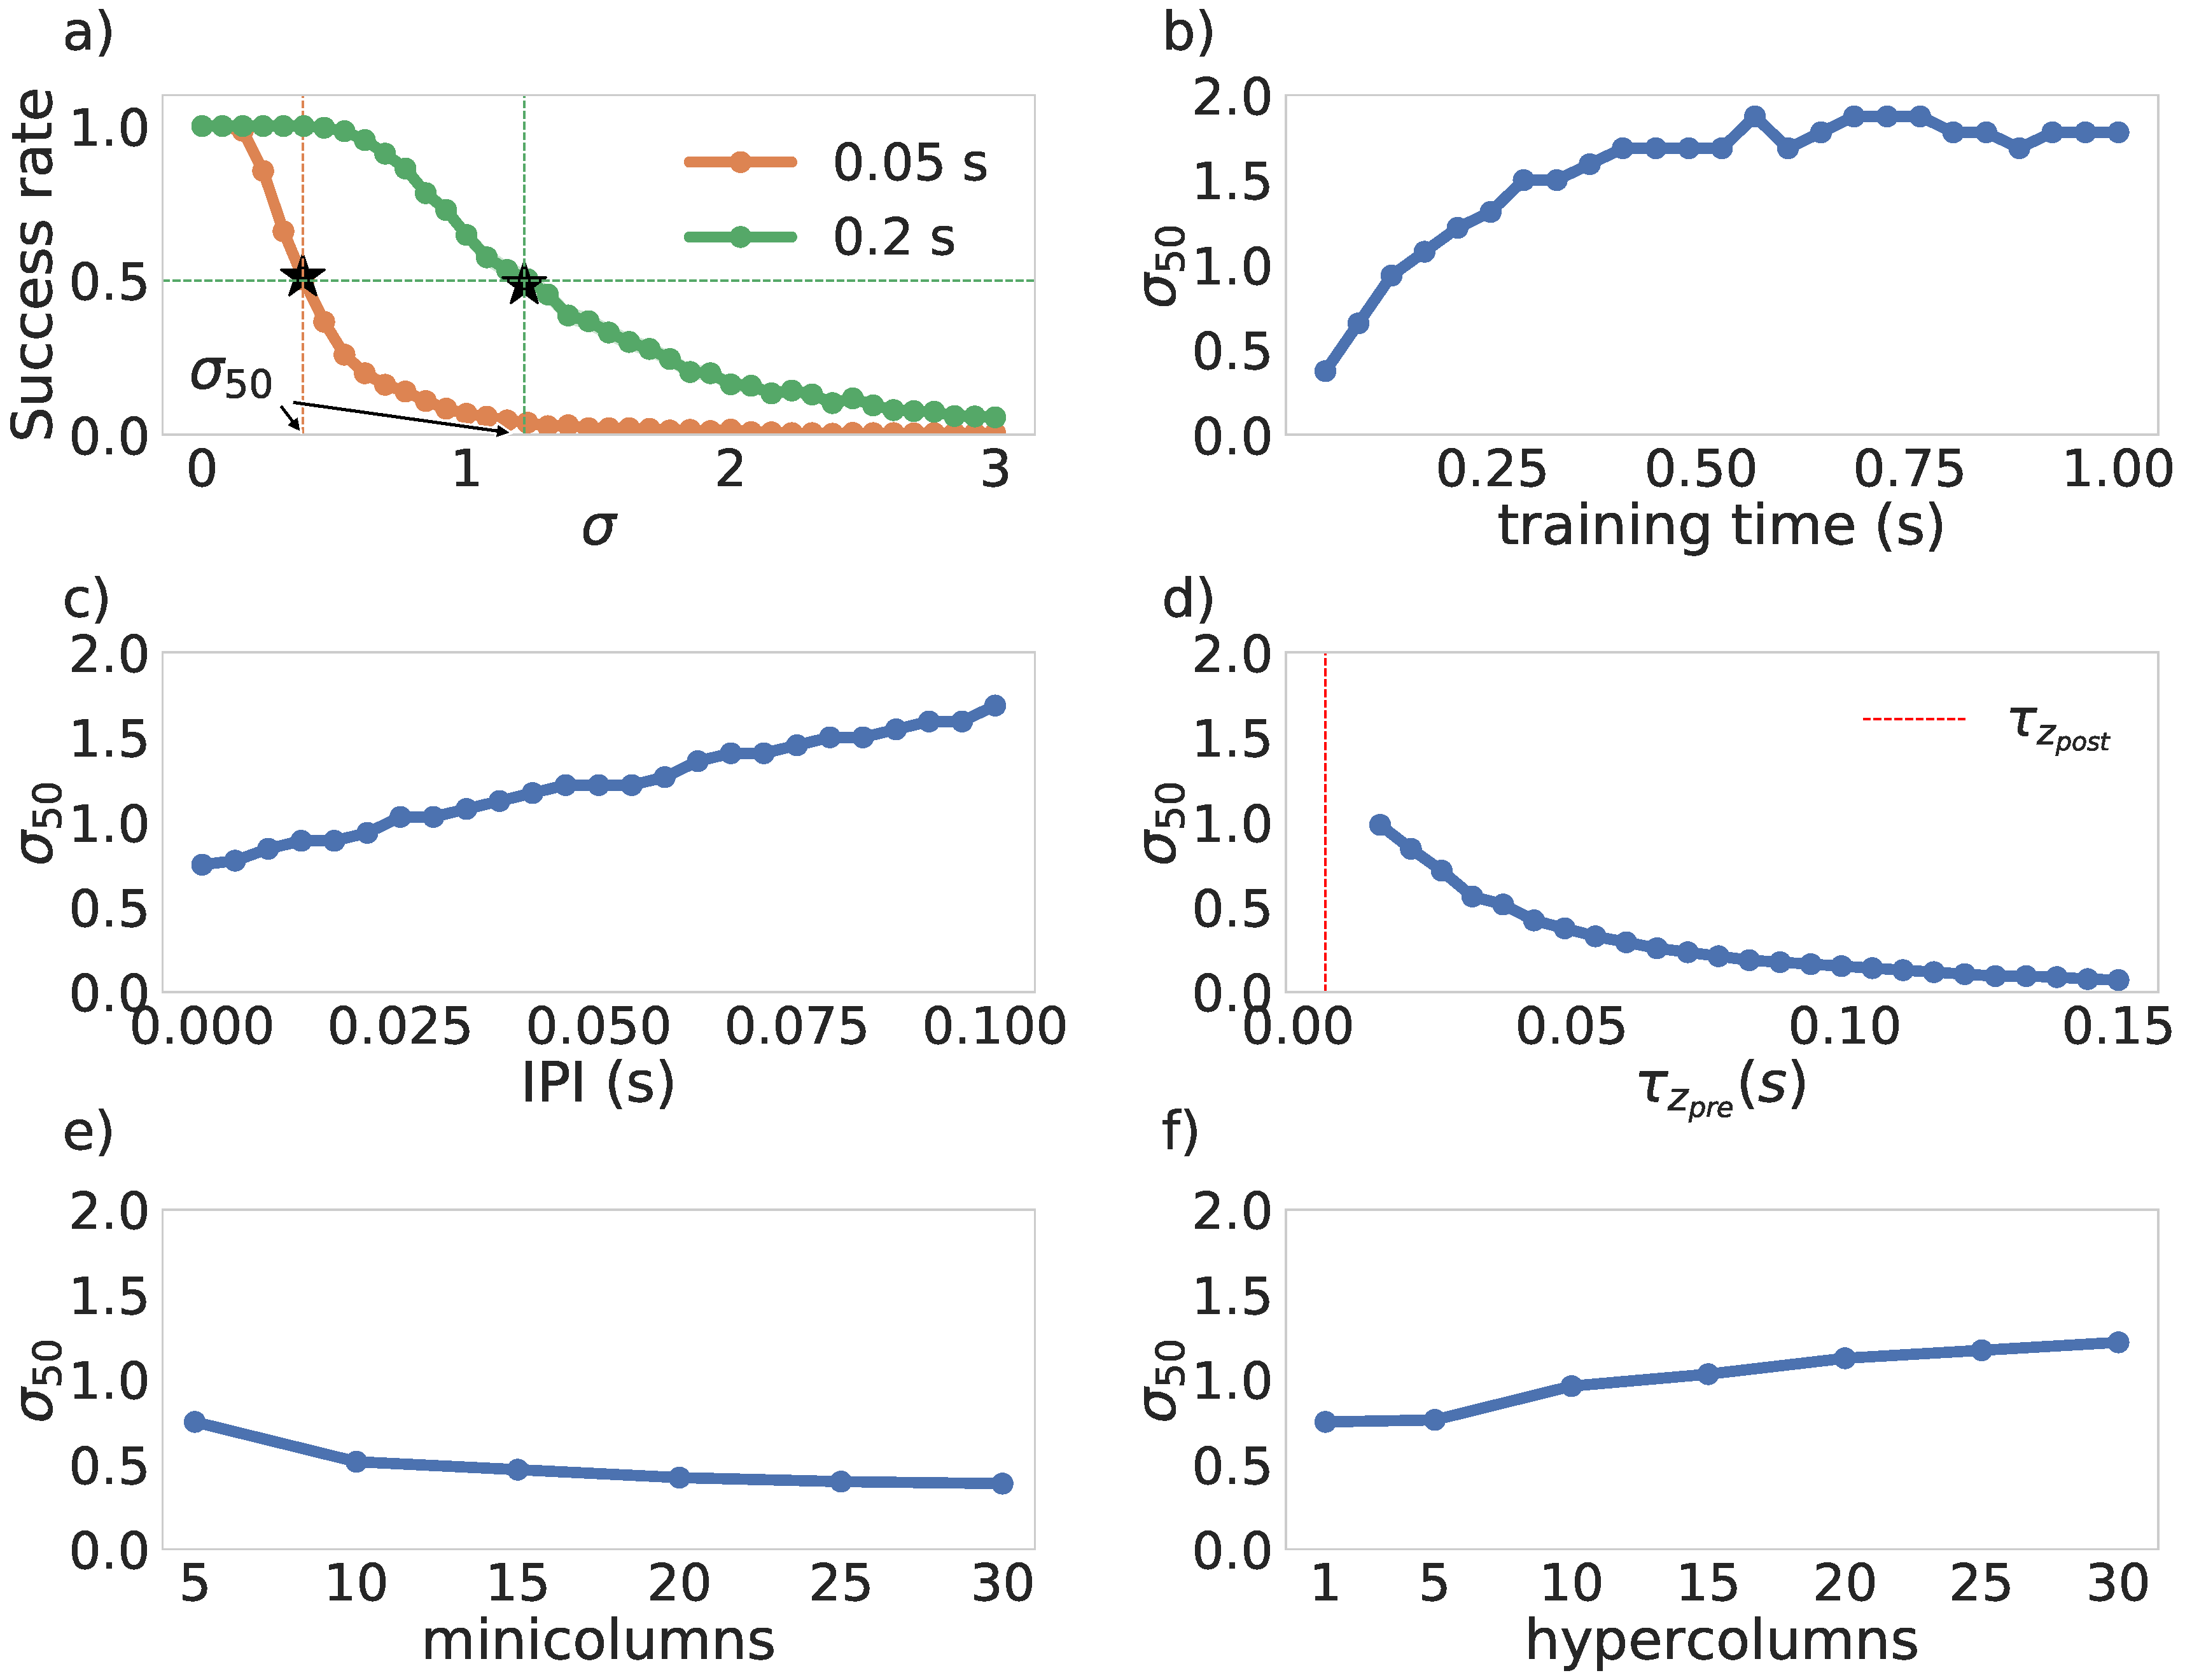
\includegraphics[scale=0.20]{noise_robustness.pdf}
\caption{Sensitivity to noise of the model that.  We use the following parameters for all the training except when the parameter itself was varied: training time $= 100 \: ms$, IPI $= 0 \: ms$, $\tau_{z_{pre}} = 25 \: ms$, $\tau_{z_{post}} = 5 \: ms$ minicolumns $=5$, hypercolumns$=1$. a) Two examples of the success vs noise profiles (training time is equal to$50 \: ms$ and $200 \: ms$). We also annotated the values of $\sigma$ at which the success rate reached its half value, we denote such values as $\sigma_{50}$. b) $\sigma_{50}$ variation with respect to the training time. c) $\sigma_{50}$ variation with respect to the IPI. d) $\sigma_{50}$ variation with respect to the $\tau_{z_{pre}}$. e) $\sigma_{50}$ variation with respect to the number of minicolumns. $\sigma_{50}$ variation with the number of hypercolumns. }
\label{fig:noise_sensitivity}
\end{figure}


\subsection{Representations}

Previous work with attractor models has shown that it is possible to store attractor states with overlapped representations \cite{meli2013modular} \cite{sandberg2002bayesian}. That is, it is possible to store two patterns in a network that share some unit activation. We test here whether is it possible to encode such overlapped patterns even when they belong to different sequences and participate in sequential processing. This is desirable first because its possibility greatly increases the storage capacity of our network and two because it greatly enriches the type of combinatorial representations that our network can process. 

We present our framework for studying both problems bellow in figure \ref{fig:rep_diagram}. In figure \ref{fig:rep_diagram}a) we show a symbolic representation of two sequences that we store in a network. The sequence one (in blue) and the sequence 2 (in red) posses patterns that share units. Concretely the pattern C and D (gray area) share the same units in the second and third hypercolumns. We then say that the sequences $1$ and $2$ have a representation overlap of $\frac{2}{3} = \frac{\text{\# hypercolumns shared}}{\text{\# total hypercolumns}}$. If we look at the sequence as a whole we see that of the six patterns in the sequence (A, B, C, D, E and F) two of them share some elements (patterns C and D or the gray area), as sequences then, we say that the patterns have a sequential overlap of 2. In short, a representation overlap is a measure of of the similarity between representations of a given number of patterns belonging two different sequences (the overlap in their basin of attraction) whereas a sequence overlap is a measure of the number of patterns in a sequence that have such similarities with another sequence. Note that whereas the representation overlap is a parameter between $0$ and $1$ the sequential overlap is an unbounded parameter as sequences can be arbitrarily long.
 
A representation overlap of $1$ (all hypercolumns share the same units in some patterns) leads us to the case of sequence disambiguation where the same pattern appears in different sequences. Sequence disambiguation requires the network to use contextual information (information from the past that is still on the system) in order to successfully recall the the two sequences.


\begin{figure}[H]
\centering
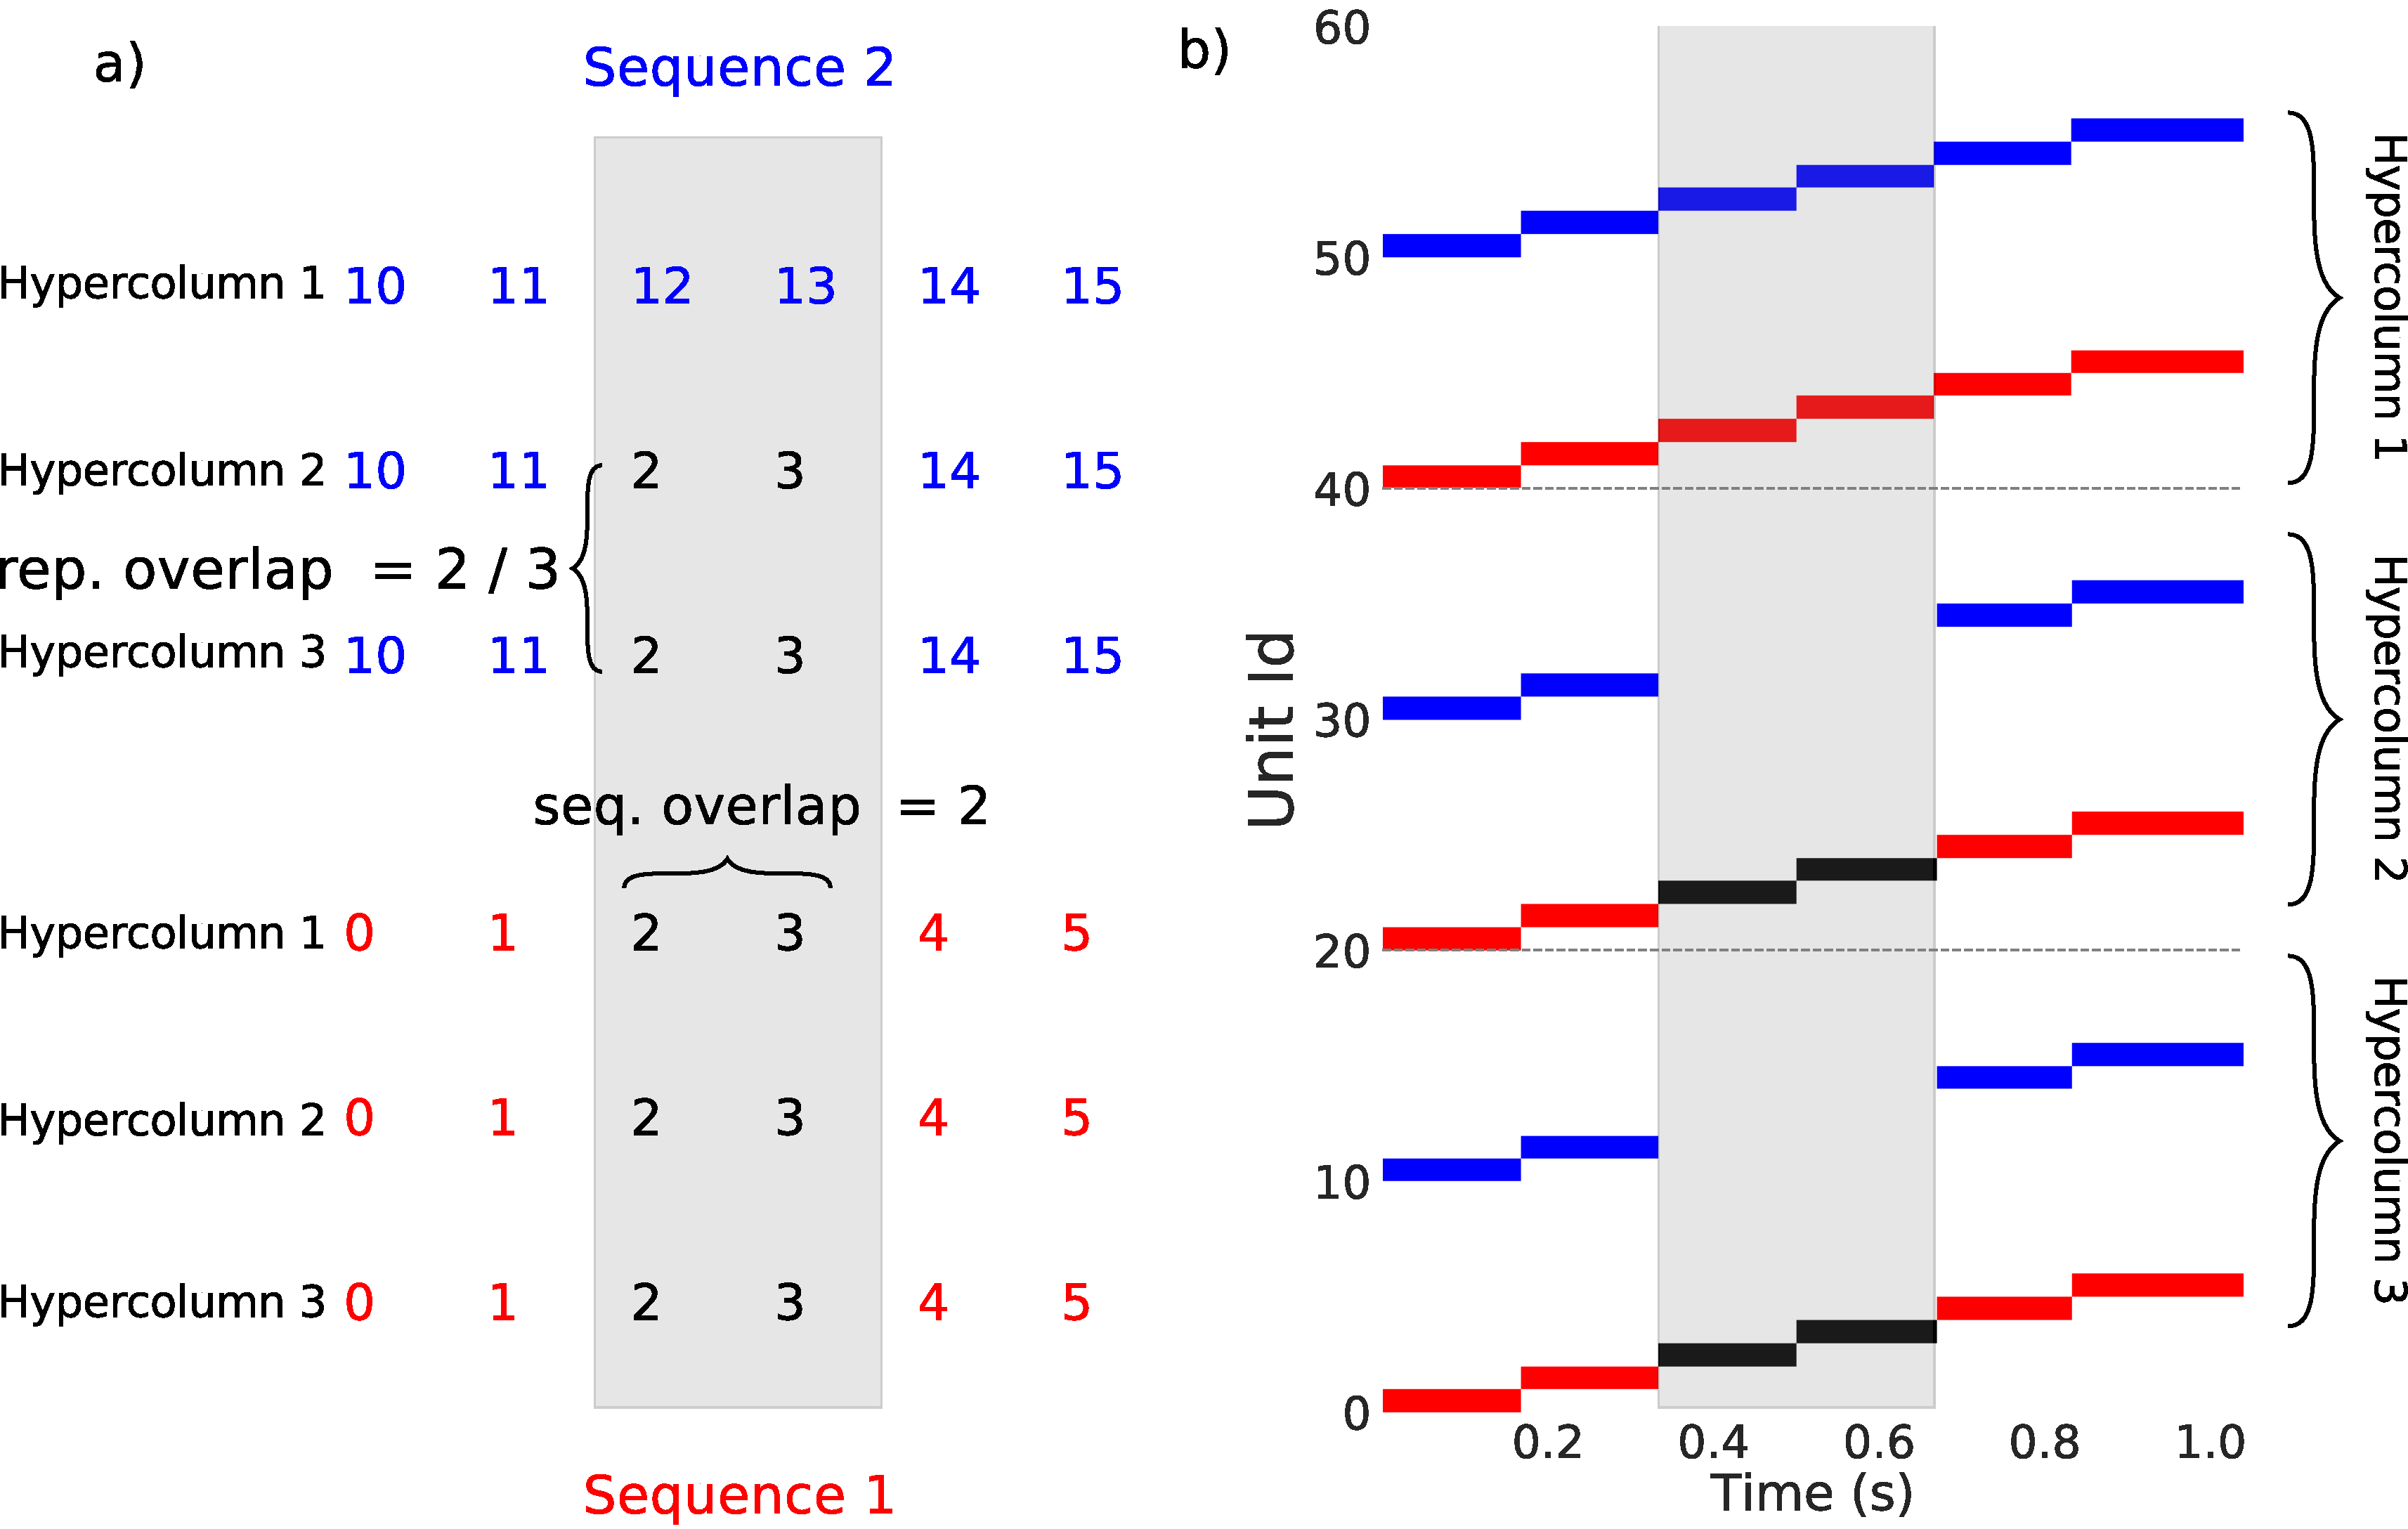
\includegraphics[scale=0.20]{rep_diagram.pdf}
\caption{Two sequences with both representation and sequential overlap. a) A symbolic representation of the sequences. Here each row is a hypercolumn and each column a pattern (patterns A, B, C, D, E, and F). The single entries represent the particular unit that was activated.  b) We show here the superposition of the recall phase for both sequences with each sequence recall emphasize by its color. We can appreciate inside the gray area that the second and third hypercolumns (sequential overlap of 2) have the same units activated (depicted in black) at the same point in the sequence reflecting again a the representation overlap of $\frac{2}{3}$. c) schematic representation of the relationship between the two stored sequences. Here each circle represents a pattern, the gray area represents the sequential overlap while the black area is the representation overlap, that is, how similar the patterns are between themselves. }
\label{fig:rep_diagram}
\end{figure}

In general the higher the representation and sequential overlaps are the harder is the task of correctly recalling the stored sequences successfully. We now show a systematic study of our network capabilities to store and recall sequences in such environment. The results are summarized in figure \ref{fig:representations}. First in figure \ref{fig:representations}a) we test whether we get correct recall for the two sequences in the zero noise condition. Besides the disambiguation regime (representation overlap equal to 1) where the overlapped patterns are completely identical the network can successfully recall overlapped sequences over a wide arrange of sequential and representation overlap parameters. However, a possible situation is that the ability of the system to solve the tasks crumbles quickly with noise. To show that this is not the case we pick four points of the space (1, 2, 3 and 4 in figure \ref{fig:representations}a)) and calculated the success vs noise profile that we show in figure \ref{fig:representations}b). We see that despite their different degrees of sequential and representational overlap the success rate vs noise profile is very similar. This shows first that the ability of the network to successfully recall sequences in this regime is not brittle and second, it leads us to suspect that the sensitivity of the system to noise may be independent of the level of representation and sequential overlap. In order to more thoroughly study the second question we calculated $\sigma_{50}$ over a whole spectrum of both sequential overlap (green horizontal curve in figure \ref{fig:representations}a)) and representation overlap (blue vertical curve in figure \ref{fig:representations}a)). We show the results in \ref{fig:representations}c)and \ref{fig:representations}d) respectively showing that sensitivity to noise profile is very similar across the parameter regime. 


The top horizontal line in figure \ref{fig:representations} is the disambiguation regime. The disambiguation capabilities of the network are due to memory effects on the dynamics. (here capacitance effects mediated by $\tau_s$). To illustrate this, we show in figure \ref{fig:representations}e) that the disambiguation capabilities of the network disappear if the attractors are encoded to last longer as the information is lost in the dynamics in those situations. Moreover, in the disambiguation regime the recall capabilities are in fact brittle as the success vs noise profile curves in figure \ref{fig:representations}f) show. The success rate decays extremely fast. This can be explained by the fact the capacitance effects of the system here are of the order of $\tau_s \sim 10 \:ms$ which make the dynamical memory extremely week. However, an interesting resonance phenomena occurs for low sequential overlap where the success rate actually increases with noise. This can be explained with the fact that the noise effectively reduces the mean $T_{persistence}$ (as shown in figure \ref{fig:noise_scheme}b) ) which makes the disambiguation power of the network strong enough to even overcome the noise. 

\begin{figure}[H]
\centering
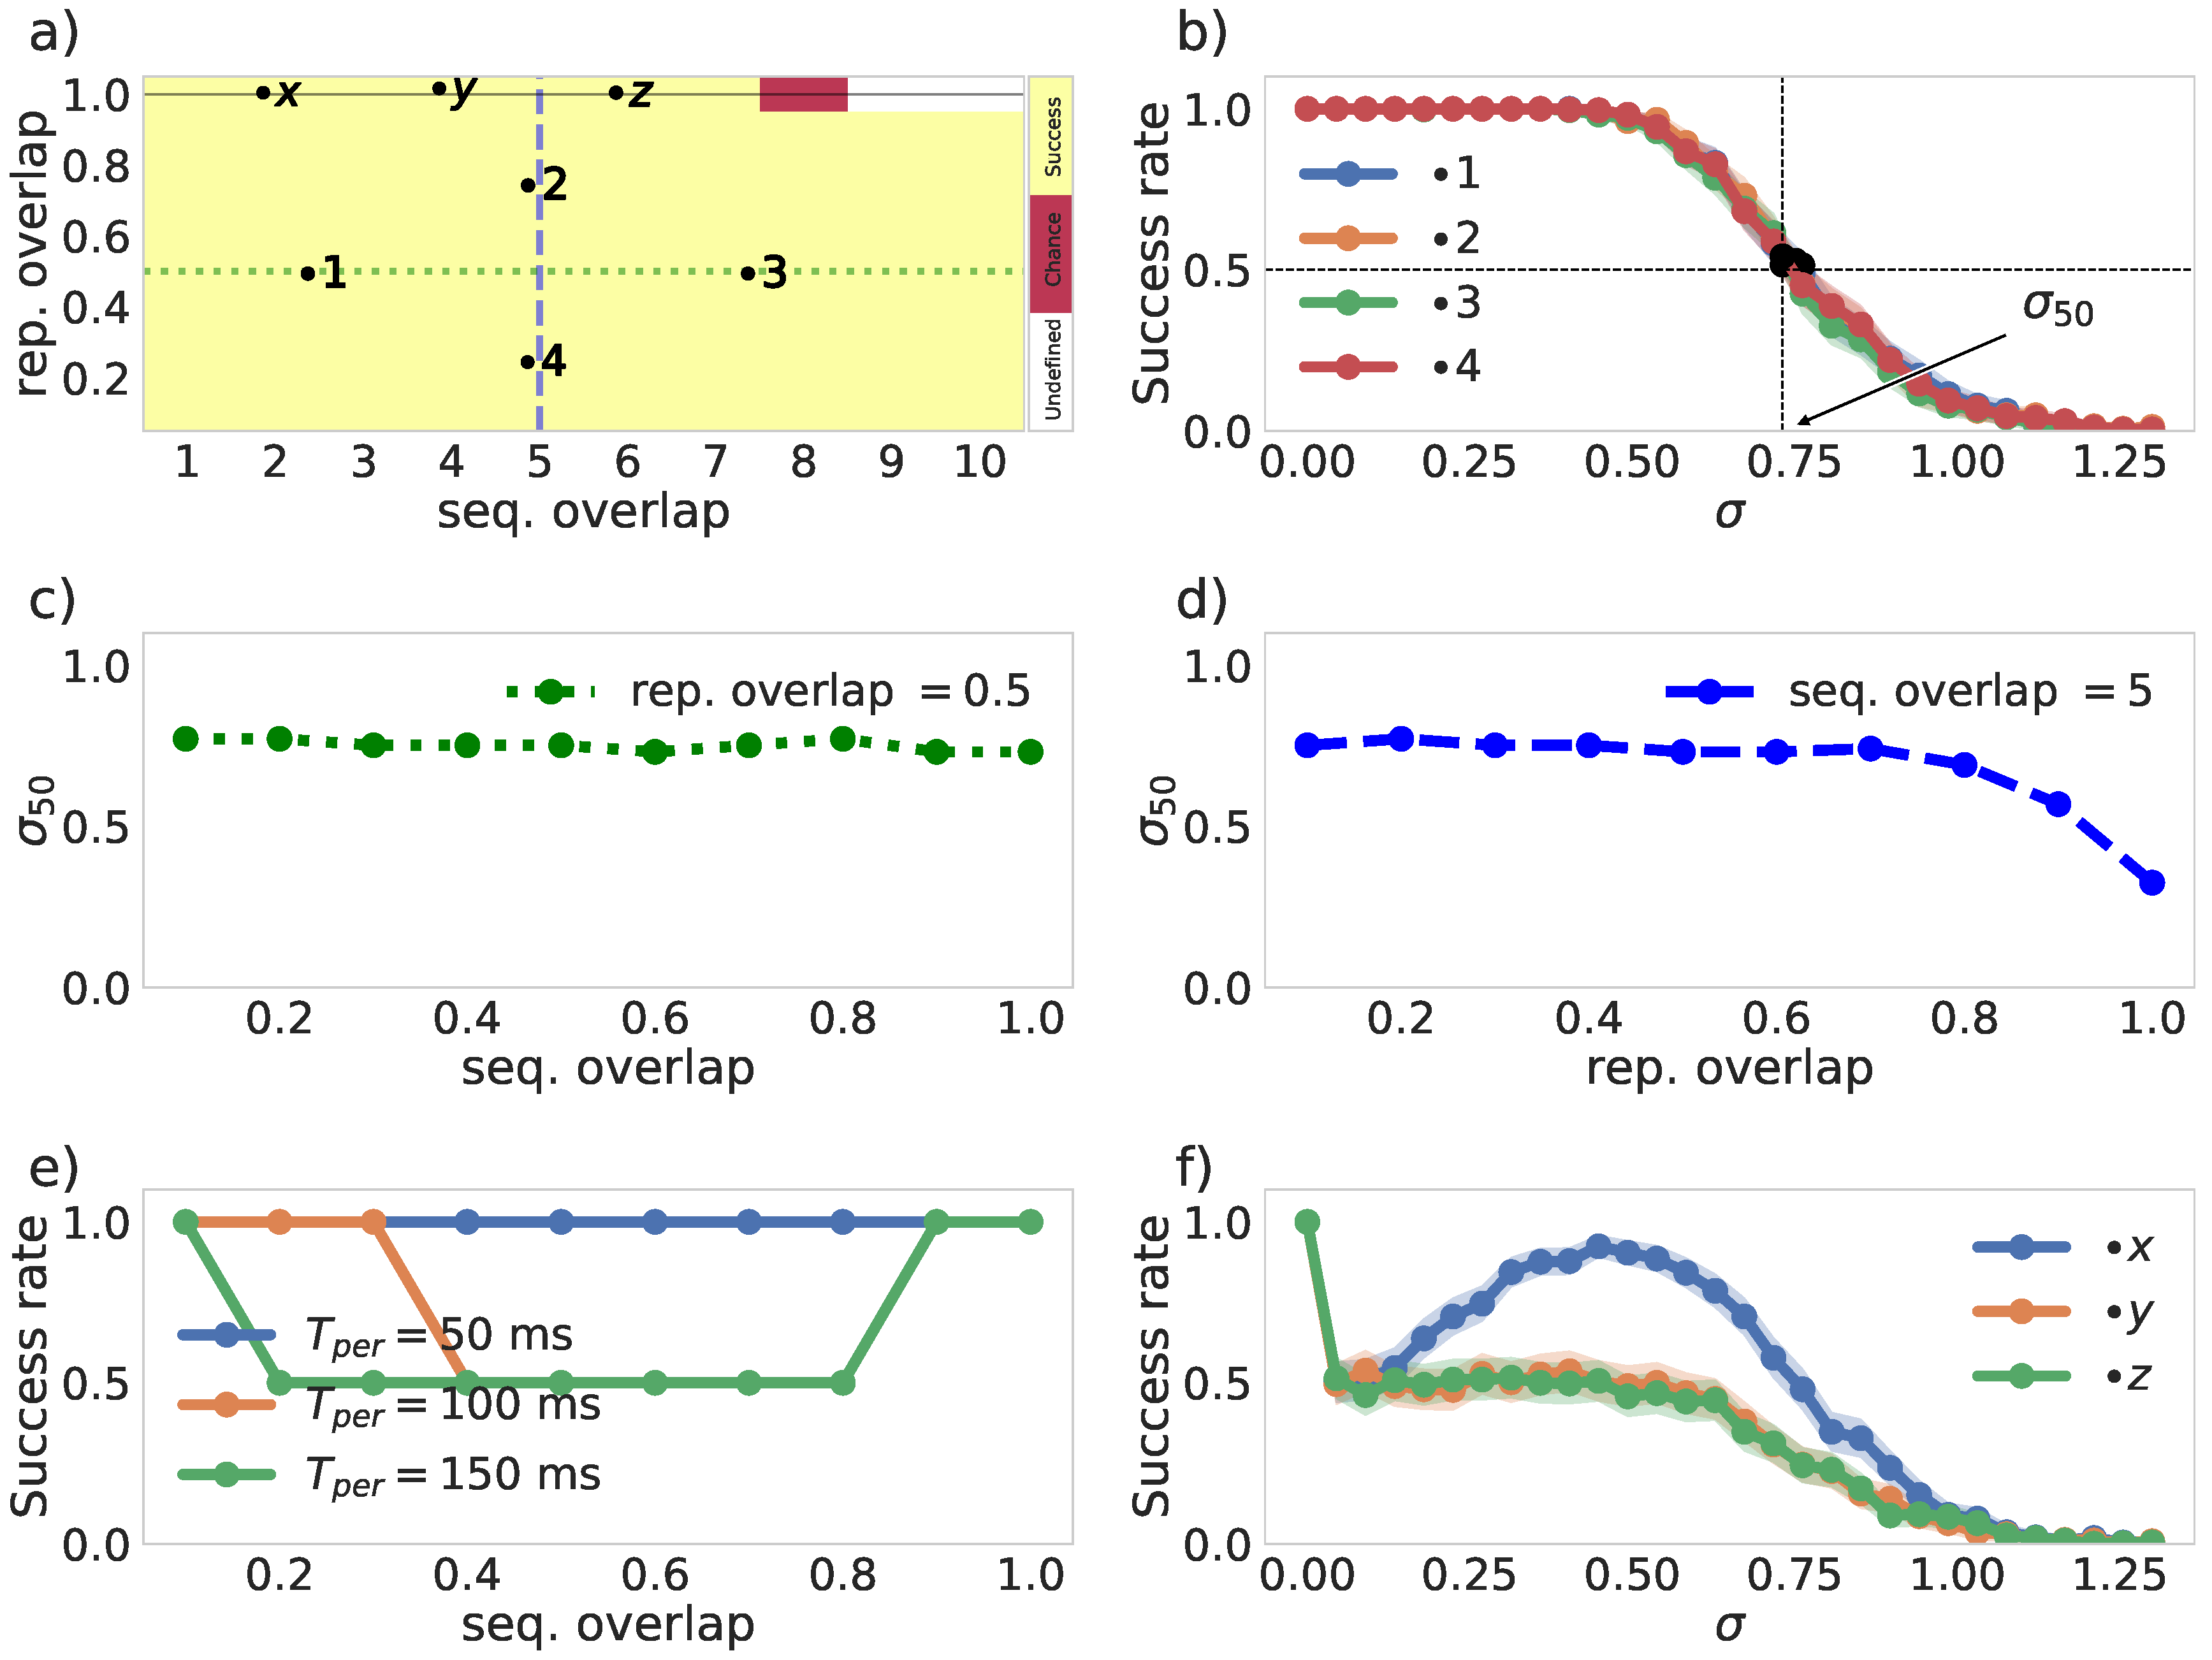
\includegraphics[scale=0.20]{representations.pdf}
\caption{A characterization of the different overlap conditions. When the parameters are not subjected to variation themselves their values are training time $= 100 \: ms$, IPI $= 0 \: ms$, $\tau_{z_{pre}} = 25 \: ms$, $\tau_{z_{post}} = 5 \: ms$ minicolumns $=20$, hypercolumns$=10$ and $T_{per}=50 \: ms$. a) success recall averaged over the two sequences for different sequential and representation overlaps. b) success rate vs noise profile for the four different points marked with numbers in a). Note that we mark the quantity $\sigma_{50}$ estimated bellow. c) $\sigma_{50}$ as a function of the sequential overlap over the green horizontal line in a). d) $\sigma_{50}$ as a function of the representation overlap over the vertical blue line in a). e) success rate in the disambiguation regime (black horizontal line in 1). f) success vs noise profile for the three different points in the disambiguation regime (a, b and c marked in 1)).}
\label{fig:representations}
\end{figure}


%\subsection{Non-homogeneous training conditions}
%
%\begin{figure}[H]
%\centering
%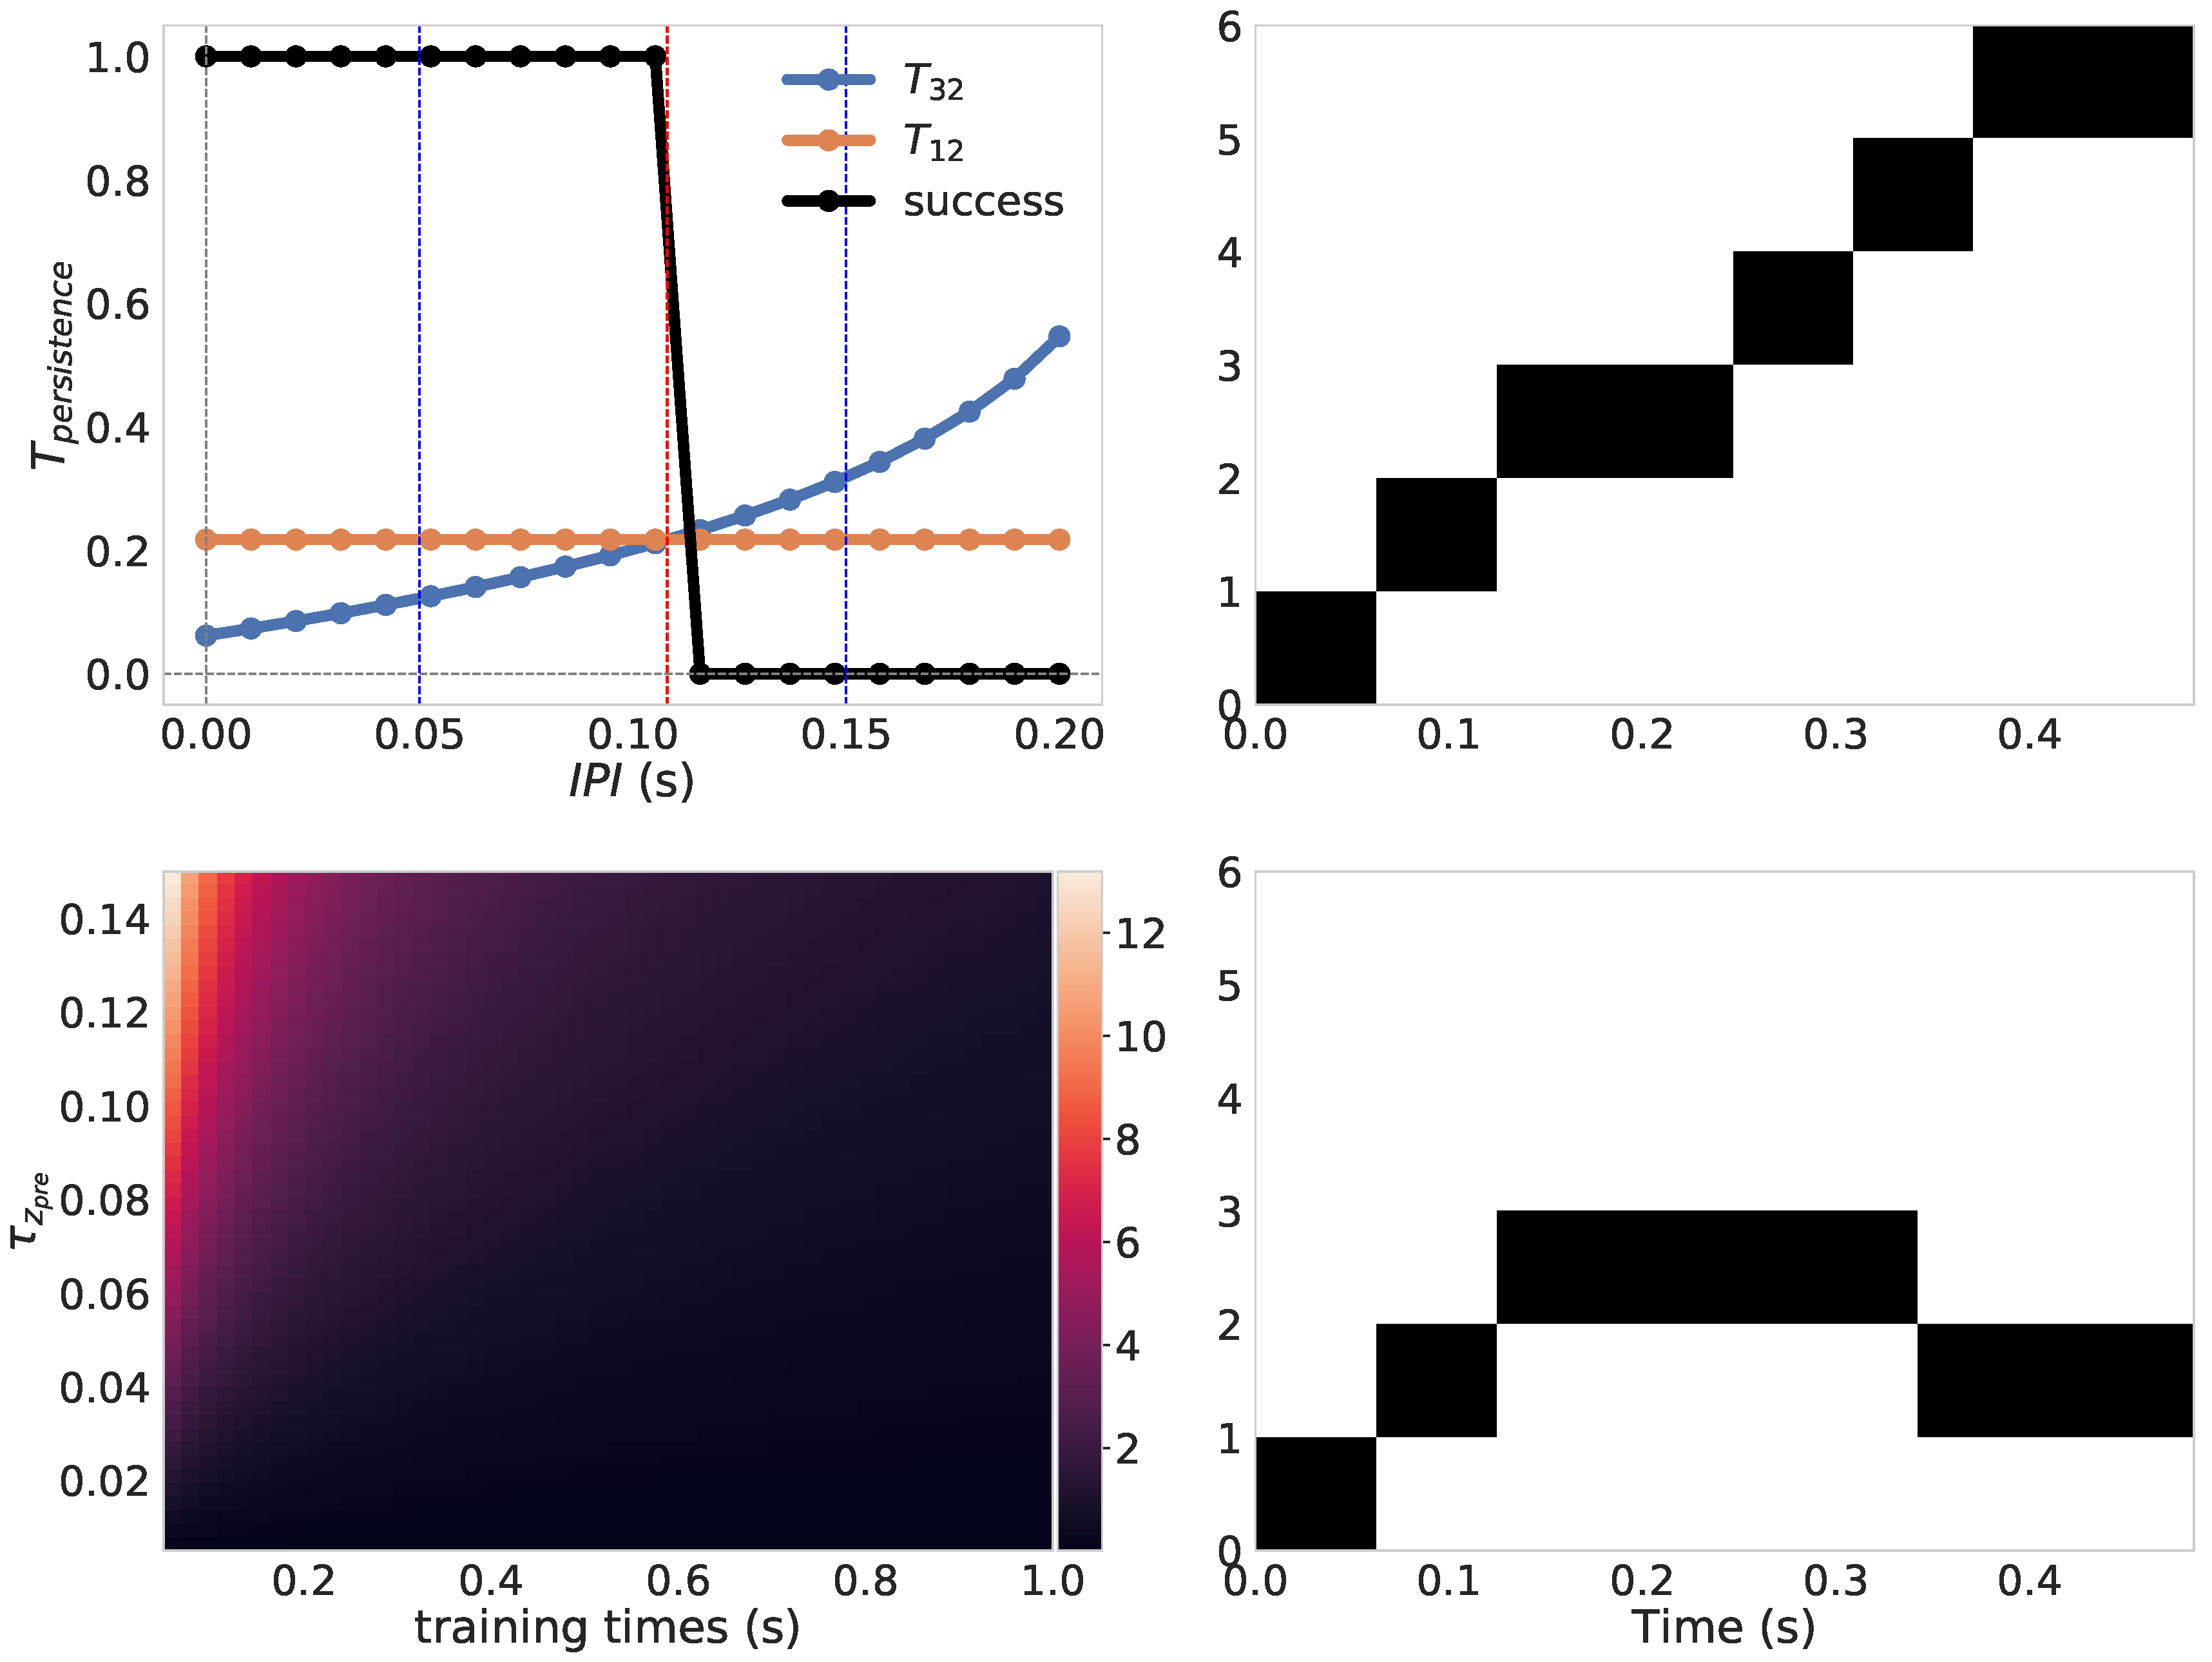
\includegraphics[scale=0.20]{ipi_non_homogenous.pdf}
%\caption{A characterization representational and sequential overlap. a) }
%\label{fig:non-homo}
%\end{figure}

\section{Discussion}

Some general pointers not in order and not well written yet.

Comparison with Phill?

Comparison of our model with Fiete, Verduzco, Murray, Silva. 

We should discuss here the biologically plausbility of the z-traces and their relationship to AMPA and NMDA 

How the problem of disambiguation may actually be robustly solved by using two different z-traces intead of one

There is evidence that the mechanisms of learning and recall  are decoupled \cite{kawai2015motor}. This is relevant because the temporal order of our system does not depend on the connectivity matrix, once it is set on stone so to speak we can control the recall with the parameters of the adaptation and the input. 

This is the point were violation of Dale Law should be addressed. 

Also maybe mentioned the fact the results are not qualitatively different with a softmax function instead of a hard-max?

Only one learning rule against multiple mechanisms, an argument of simplicity. Other models have to work with an interplay of associative learning rules and heterosynaptic ones to solve the problem of positive feedback leading the network into a runaway domain. The BCPNN learning rules takes care of this.

How do this models play with SORN, Liquid State Machines type of models where the dynamics keep information (MINAI paper). Answer, you can achieve the same with this model, the other model seems more complex.

Hawkins mechanisms of sequence disambiguation. We do basically the same, but he calls a highly overlapped spatial representation of a pattern the same representation, there is a contextual code based on a population code that solves disambiguation in real time. 

Further work. 1) Non-homogeneus protocol. 2) Calculation of pattern storage. 3) Learning of precise control of time.


\section{Methods}

\subsection{Pattern Activation}
We define pattern activation in the following way. First we calculate a vector with the cosine similarity between all the patterns stored and the network state $\mathbf{o}$ at every point in time $sim_i(t) = \frac{\mathbf{pattern_i} \bullet  \mathbf{o}(t)}{\Vert \mathbf{pattern_i} \Vert \Vert \mathbf{o}(t) \Vert}$. Note that this will give a time series for every element of the vector $sim$. Second we form a times series with the most similar pattern to the network state at every point in time by choosing the pattern index with the most similarity $winner(t) = \max \: \mathbf{sim(t)}$. This time series is as long as the number of points in time that the simulation possess. Finally, in order to get the sequence of activations we considered as active any pattern that was the winner for longer than  $T_{winning} \:$ which was set to $T_{winning} = \tau_s = 10.0 \: ms$ unless otherwise specified.   

\subsection{Recall Protocol}
For the recall protocol we briefly activate the complete pattern for $\tau_s = 10 \: ms$. The network is then free to evolve according to its internal dynamics. The sequence (0, 1, 2, 3) is considered to be correctly recalled if by activating the first pattern in it (pattern 0) all the others patterns on the sequence are activated in the specific order that they were stored. Given that for many possible tasks it suffices that the network state ends in the correct pattern or that only a part of the sequence is recalled correctly our success criteria may appear overly narrow. However in making this choice we have traded generality for specificity with the aim of establishing a lower bound for the correct recall conditions of sequence processing.


\subsection{Calculation of Persistent Time}
In order to calculate $T_{persistence}$ of pattern $i$ we calculated the difference between the time $t_1$ at which pattern $i$ became activated ($winner(t_1) = i$) to the first point in time at which it was not ($winner(t_2) \neq i$). Then we simply defined $T_{persistence} = t_2 - t_1$.

As shown in equation \ref{eq:persistent_times} the persistent time depends on both the weight and bias differences $\Delta w_{next} = w_{self} - w_{next}$ and $\Delta \beta = \beta_{self} - \beta_{next}$ and the adaptation gain $g_a$. This allow us to  set the persistent time of an attractor to any desired value by adjusting the adaptation gain with the formula $g_a = \frac{(\Delta w_{next} + \Delta \beta)(1 - r)}{1 - r - e^{\frac{T_{persistence}}{\tau_a}}}$. We use this adjustment to control for $T_{persistence}$ after training in order to decouple the effects of training from the ones of the persistent time in the recall phase. 

\subsection{Training Protocol}
For our training protocol we created a time series  $\mathbf{s}(t)$ to represent the input. $\mathbf{s}(t)$  encodes the information about the training time and the inter-pulse interval. We then performed off-line batch learning of the parameters using the integral formulation of the training equations above.

\begin{align}
z(t) &= \frac{1}{\tau_z } \int_{-\infty}^{t} s(\tau) e^{-\frac{t - \tau}{\tau_z}} d\tau \label{eq:flitering}  \\
p_i(t) &= \frac{1}{t}\int_0^{t} \underset{post}{z_i}(\tau) d\tau  \label{eq:bcpnn_off_line_prob} \\
p_{ij}(t) &= \frac{1}{t}\int_0^{t} \underset{post}{z_i}(\tau) 
\underset{pre}{z_j}(\tau) d\tau \label{eq:bcpnn_off_line_joint} 
\end{align}

Where we have calculated two $z$ traces, one for $\tau_{z_{pre}}$ and the other for $\tau_{z_{post}}$. The limits of the integrals were selected to coincide with the total duration of all the input. After we have the values of the probability traces we calculated $w$ and $\beta$ by using the BCPNN rule in equation \ref{eq:bcpnn}.

For training the two sequences with the overlapped representations we created a time series with the sequences in succession but separated among them by $1s$. This ensured the training protocol were uncoupled from each other.



\subsection{Noise}
We added noise in the system as an injection of white noise with variance $\sigma_{in}$ into the system at every time step. However, we characterized the system in terms of the steady state standard deviation that the system would have it it was an Ornstein–Uhlenbeck (OU) process given by $\sigma_{out} = \sqrt{\frac{\tau_s}{2}} \sigma_{in} \sim 0.07 \sigma_{in}$. The rational behind this choice is that $\sigma_{out}$ will be the actual standard deviation that the current $s$ in equation \ref{eq:current} will be subjected to precisely this standard deviation. It is important to say that thanks to the separation of times scales ($\tau_s \ll \tau_a$) the system behaves mostly as an OU process and is only the winner-take-all dynamic around the transition points that deviates the system from it as it can be appreciated in figure \ref{fig:noise_scheme}a). Throughout this work we use $\sigma = \sigma_{out}$ unless otherwise stated. 

We calculated the success rate by simply averaging how many of a given number of trials successfully recalled the sequence. In order to quantify the uncertainty over our estimates for the success rate for different degrees of noise we utilized the Wald method to provide the $95 \% $ confidence intervals for the success rate estimates:

\begin{align} 
\hat{p} \pm 1.96\sqrt{\frac{\hat{p}(1 - \hat{p})}{N_{obs} }} \label{eq:confidence}
\end{align}

For this work we mostly used $N_{obs}=1000$ and therefore we have approximately $\hat{p} \pm 0.0134$ or deviations of $1 \%$.  



\subsection{Calculation of Noise Sensitivity}
In order to systematically characterize how different parameters of our training protocol affect the sensitivity of the resulting network to noise we calculated $\sigma_{50}$. We defined $\sigma_{50}$ as the  value of $\sigma$ for which the probability of correctly recalling a given sequence is $\frac{1}{2}$. Finding such $\sigma$ is a instance of the Stochastic Root Finding Problem \cite{pasupathy2010choosing}. To estimate this we have used the naive bisection algorithm for deterministic functions by using the averages as estimates of the actual values. We stopped the algorithm as soon as the success rate corresponding to our estimate of $\sigma_{50}$ was contained in the Wald confidence interval as presented in \ref{eq:confidence}. As a validation of the algorithm ability to find the  correct value we calculated the success rate that we found at $\sigma_{50}$ as we show ther figure \ref{fig:noise_calibration} of the appendix. We find that the algorithm consistently finds a value of $\sigma_{50}$ that fulfills the criteria of the success rate being $\frac{1}{2}$. That said, in order to find a more standard statistical measure of the error in $\sigma_{50}$ we would require to perform an amount of estimations of $\sigma_{50}$ that surpasses our current computational capabilities. We believe though that the purpose of estimating the overall way in which the noise sensitivity depends on the training protocol is accomplished by our method. 

In figure \ref{fig:appendix_noise_sensitivity} in the appendix we also characterized the variation of $\sigma_{75}$ and $\sigma_{25}$  in order to have a more thorough analysis. The trends overall agree with the analysis in figure \ref{fig:noise_sensitivity}.  




\section{Apendix}
\subsection{Analytical solution}
We can solve the deterministic equations analytical with the method of undetermined coefficients. There are two conditions, the unit that is active, and the unit that is not. 


\begin{align} 
s(t) &= I_{fix} - g_a\left(\frac{C_{charge}}{1 - r} \right) e^{-\frac{t}{\tau_a}} + \left(s_0 - I_{fix} + g_a \left( \frac{C_{charge}}{1 - r}\right)\right)e^{-\frac{t}{\tau_s}} \label{eq:deterministic_solution}\\
\underset{acti}{s(t)} &= \beta + w - g_a + g_a \left(\frac{1 - a_0}{1 - r}\right) e^{-\frac{t}{\tau_a}} + \left(s_0 - \beta - w + g_a - g_a \frac{1 - a_0}{1 - r}\right) e^{-\frac{t}{\tau_s}}  \\ 
\underset{inact}{s(t)} &= \beta + w - g_a \left( \frac{a_0}{1 - r} \right) e^{-\frac{t}{\tau_a}} + \left(s_0 - \beta  - w  + g_a \left( \frac{a_0}{1 - r} \right) \right) e^{-\frac{t}{\tau_s}} 
\end{align}

Where $r=\frac{\tau_s}{\tau_a}$ and $C_{charge}=a_0$ for the non-active case and $C_{charge} = a_0 - 1$ for the active case. Same for $I_{fix}=\beta + w$ for the non-active case and $I_{fix} = \beta + w - g_a$ for the active case. 

\subsection{Role of the z-traces' Time Constants}
\begin{figure}[H]
\centering
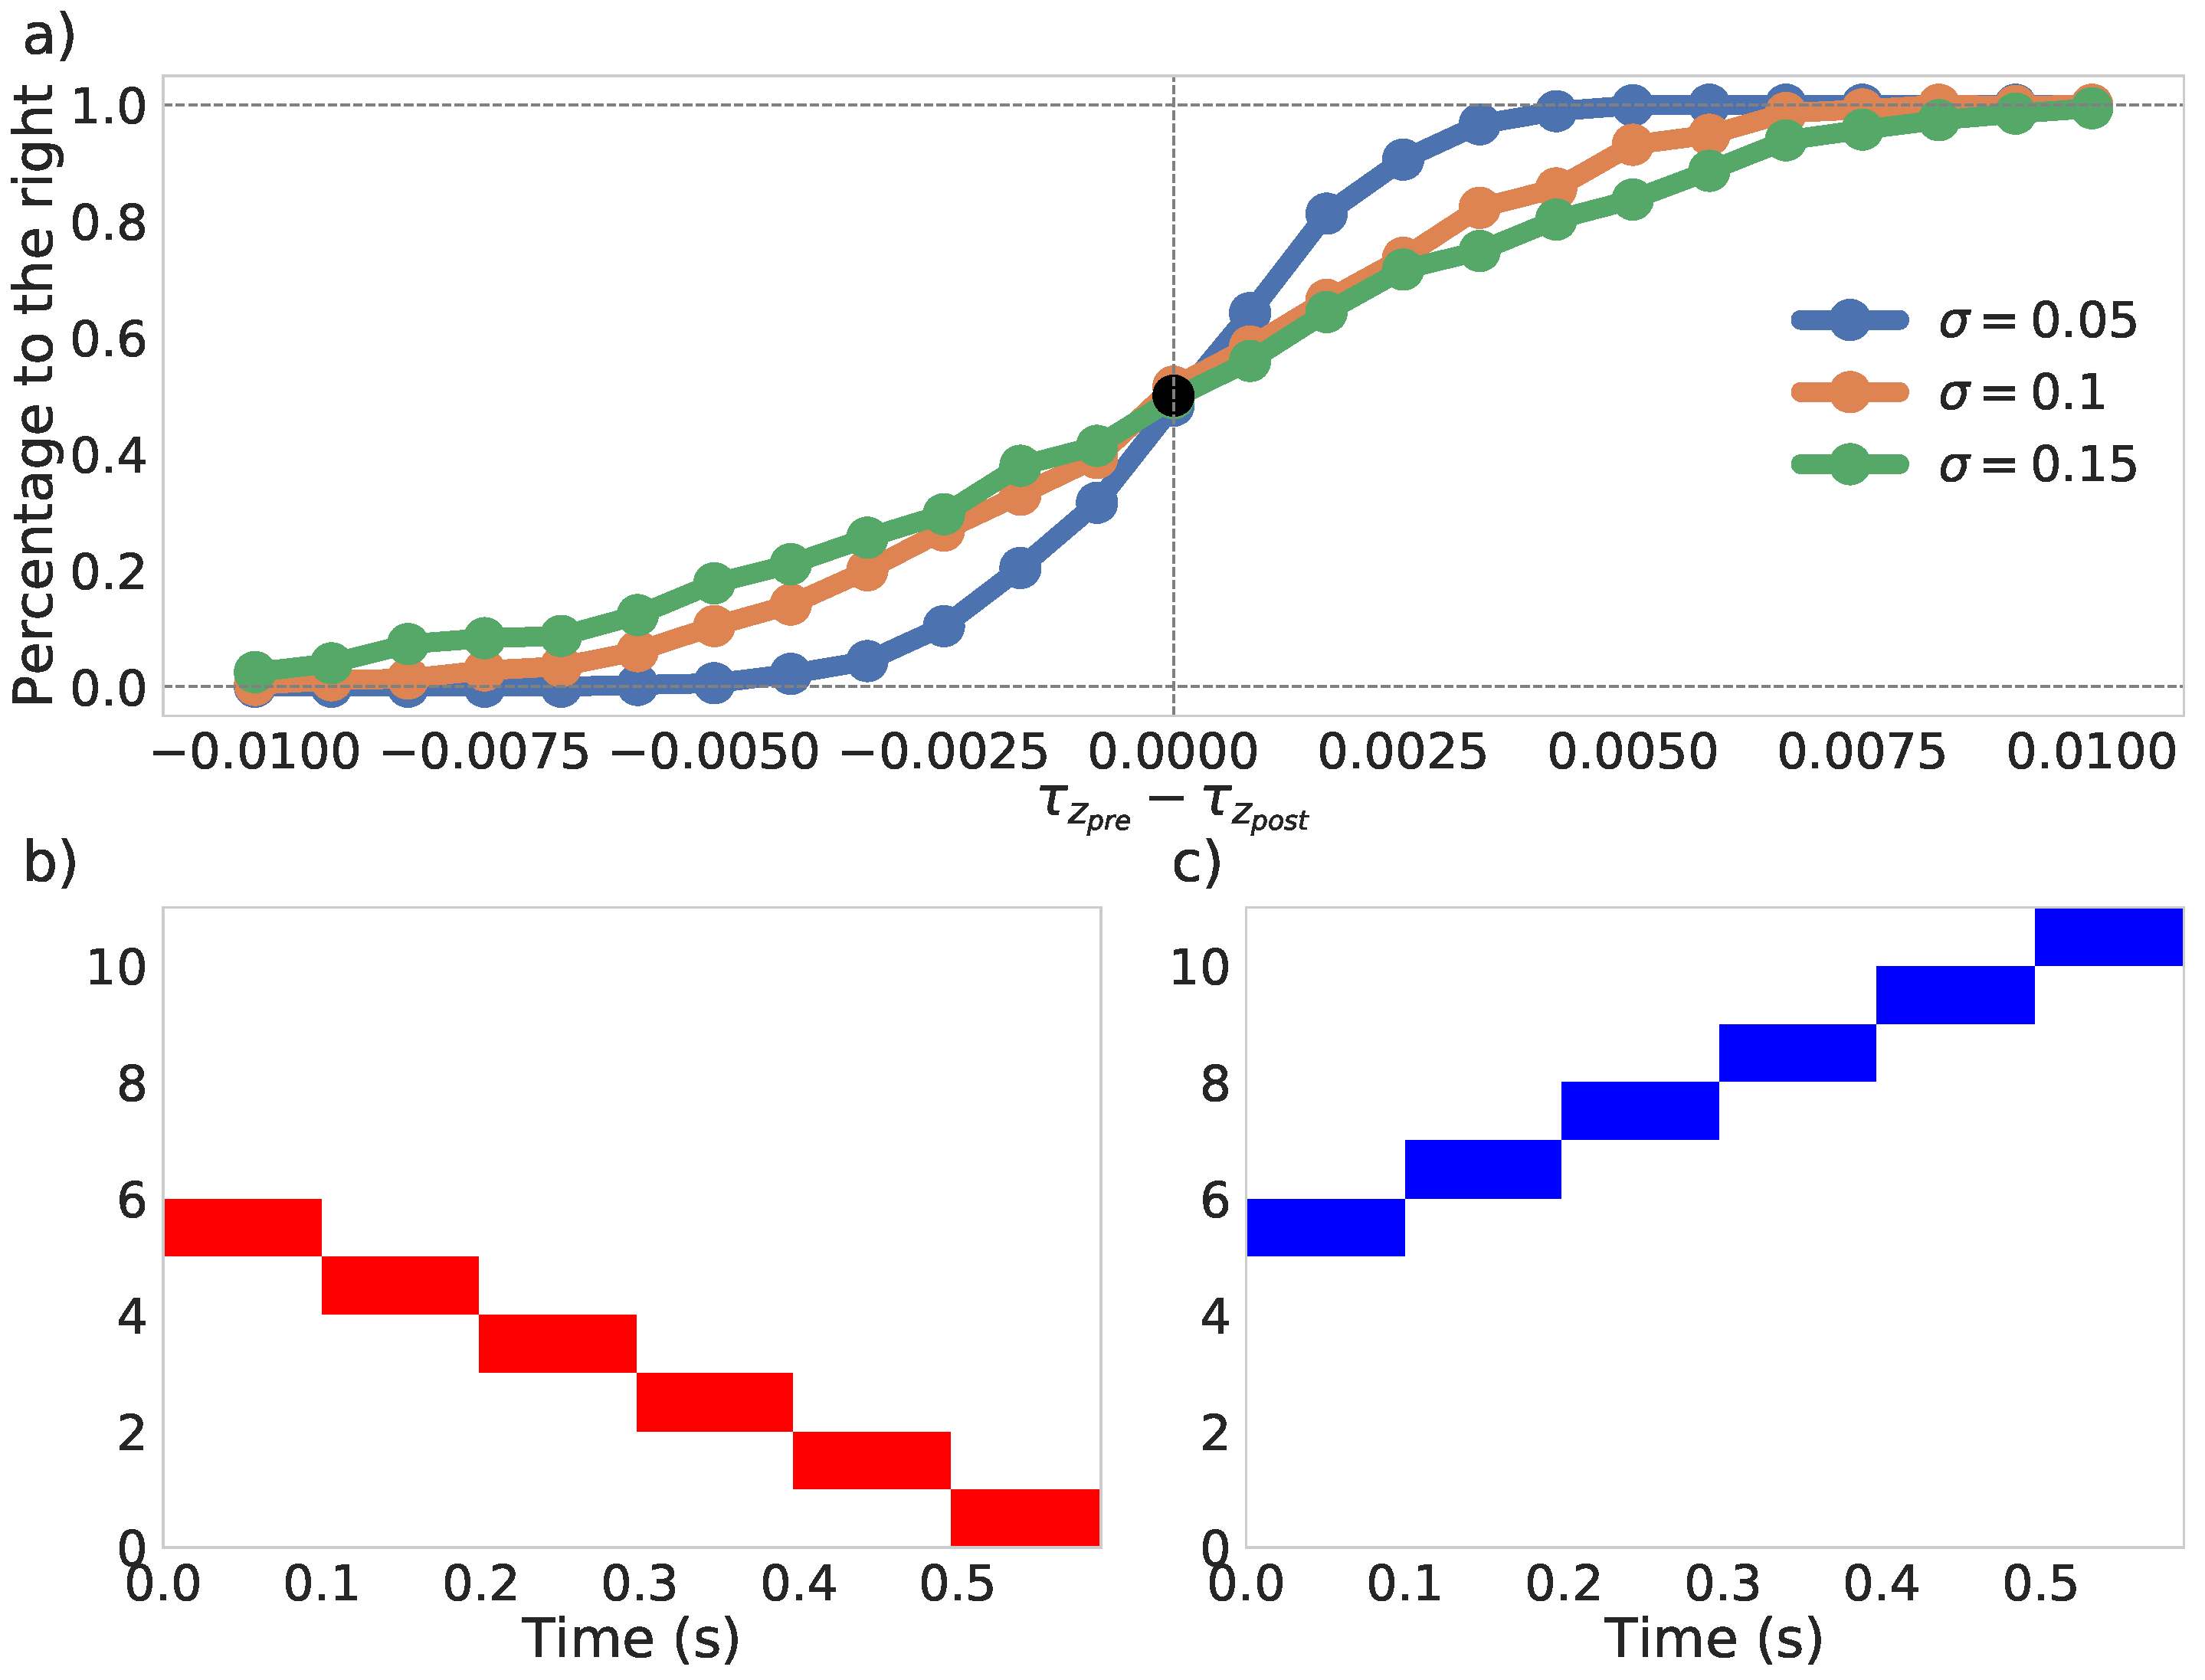
\includegraphics[scale=0.20]{asymmetry.pdf}
\caption{$\tau_z$ effects on sequence recall direction. }
\label{fig:z-assymetry}
\end{figure}

\subsection{Time encoding}
\begin{figure}[H]
\centering
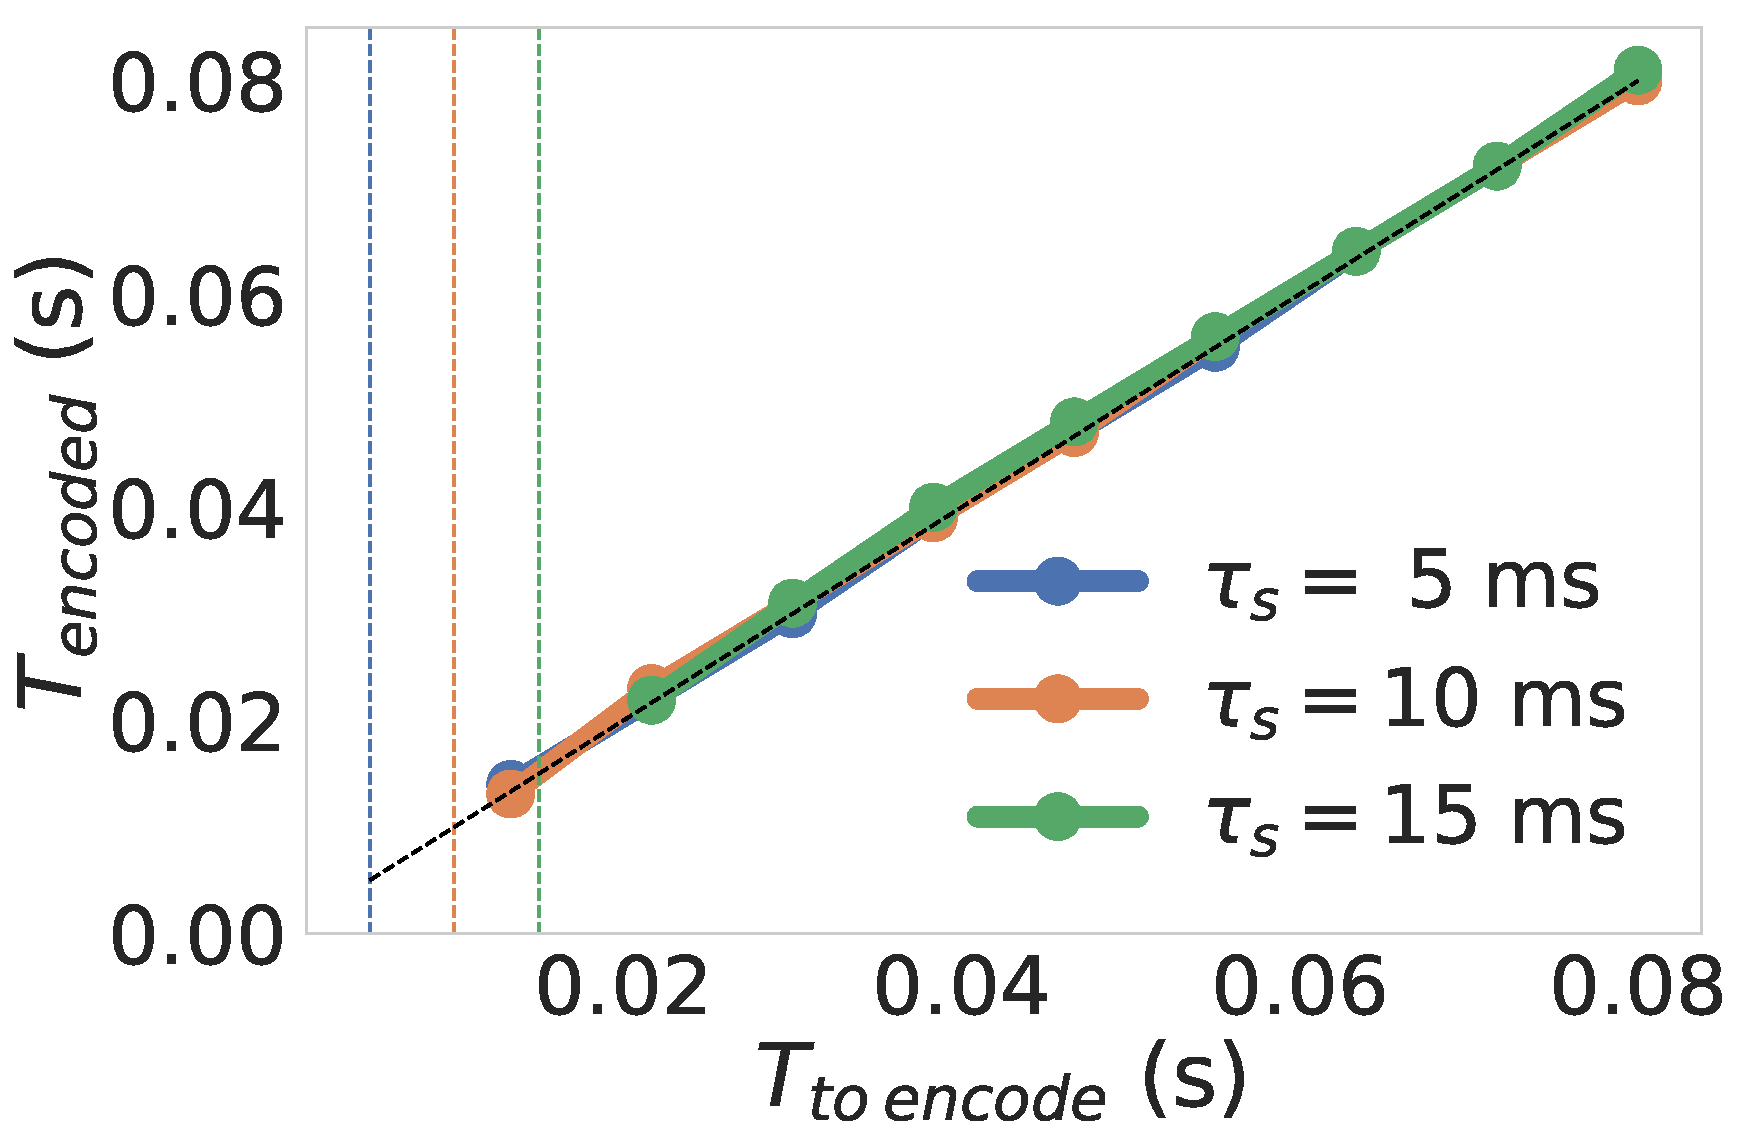
\includegraphics[scale=0.40]{time_encoding.pdf}
\caption{Minimal time encoding. In the x axis we have a particular time that we wish we encode as the persistent time of an attractor. In the y axis we have the time that is actually encoded through the method of fixing the adaptation gain. The leftmost points indicate the minimal possible encoding and after that the time was not encoded successfully. Vertical dashed lines represent the value of $\tau_s$ used for the simulation. We chose the value the middle value of $\tau_s=10 \: ms$  as our $T_{wining}$ (the minimal amount of activation necessary to appear on the sequence).}
\label{fig:min_time_encoding}
\end{figure}

\subsection{Sensitivity calibration}

\begin{figure}[H]
\centering
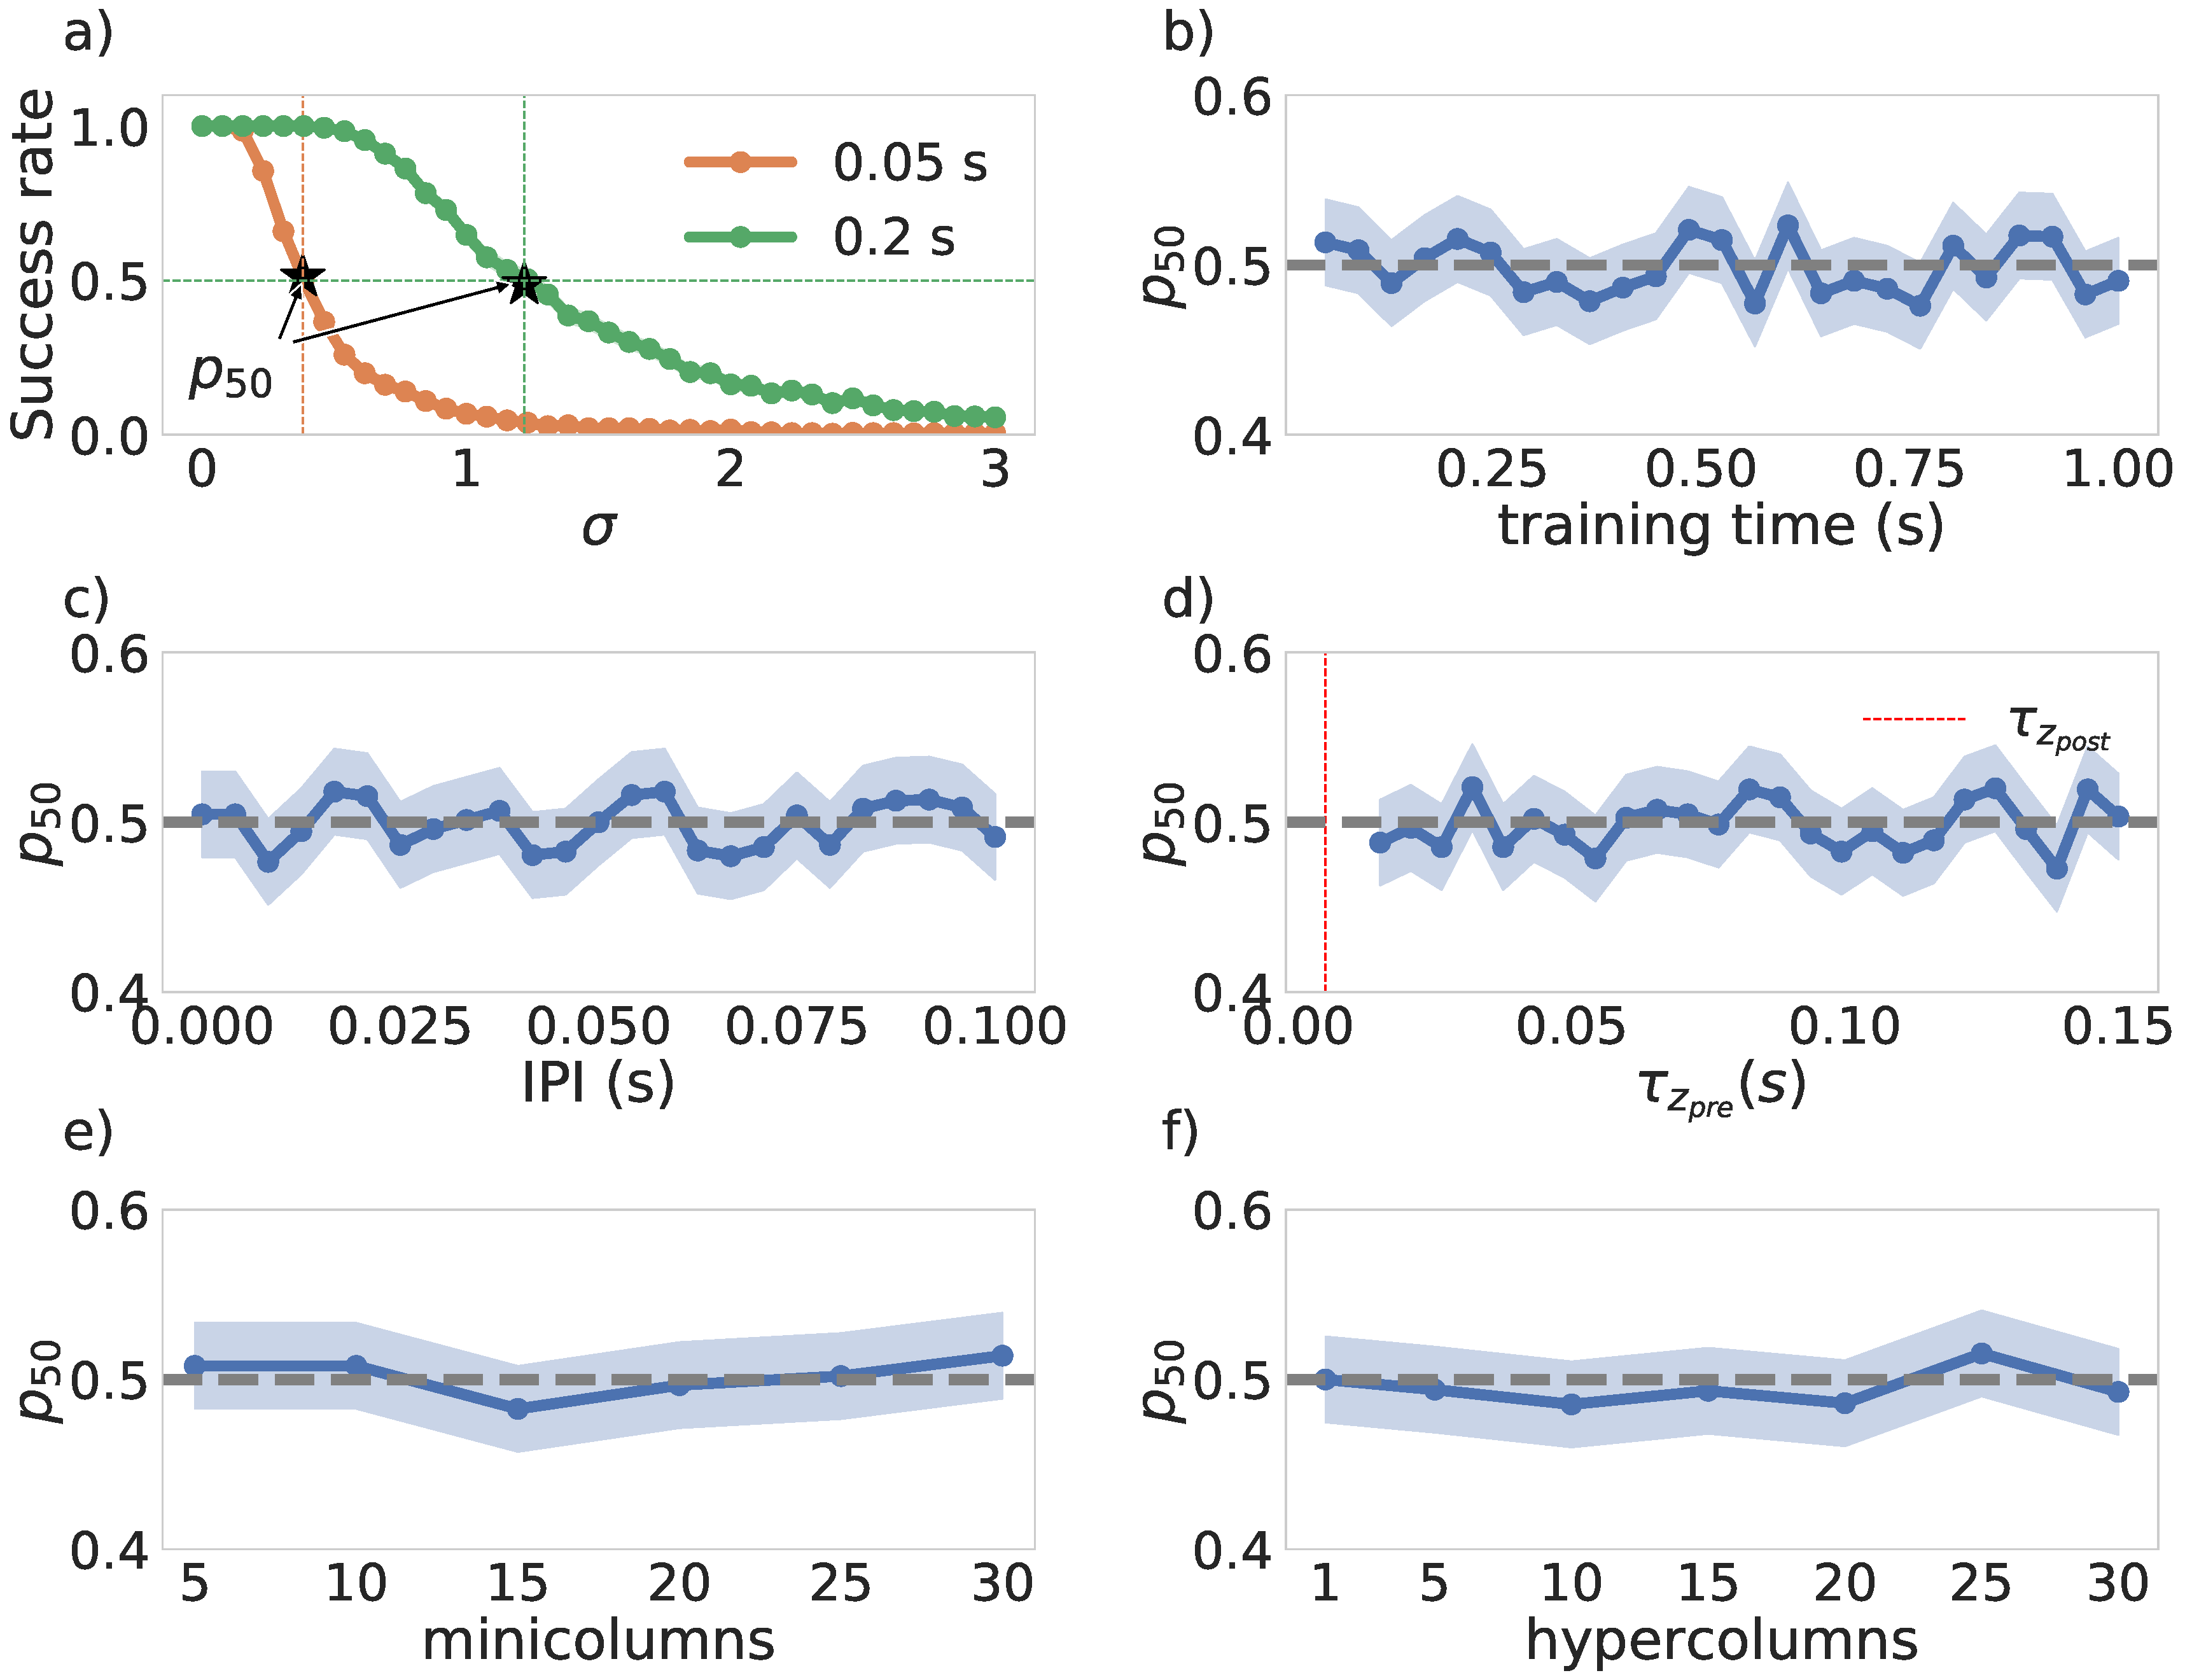
\includegraphics[scale=0.20]{noise_estimates.pdf}
\caption{Calibration of $\sigma_{50}$ estimation.}
\label{fig:noise_calibration}
\end{figure}

\begin{figure}[H]
\centering
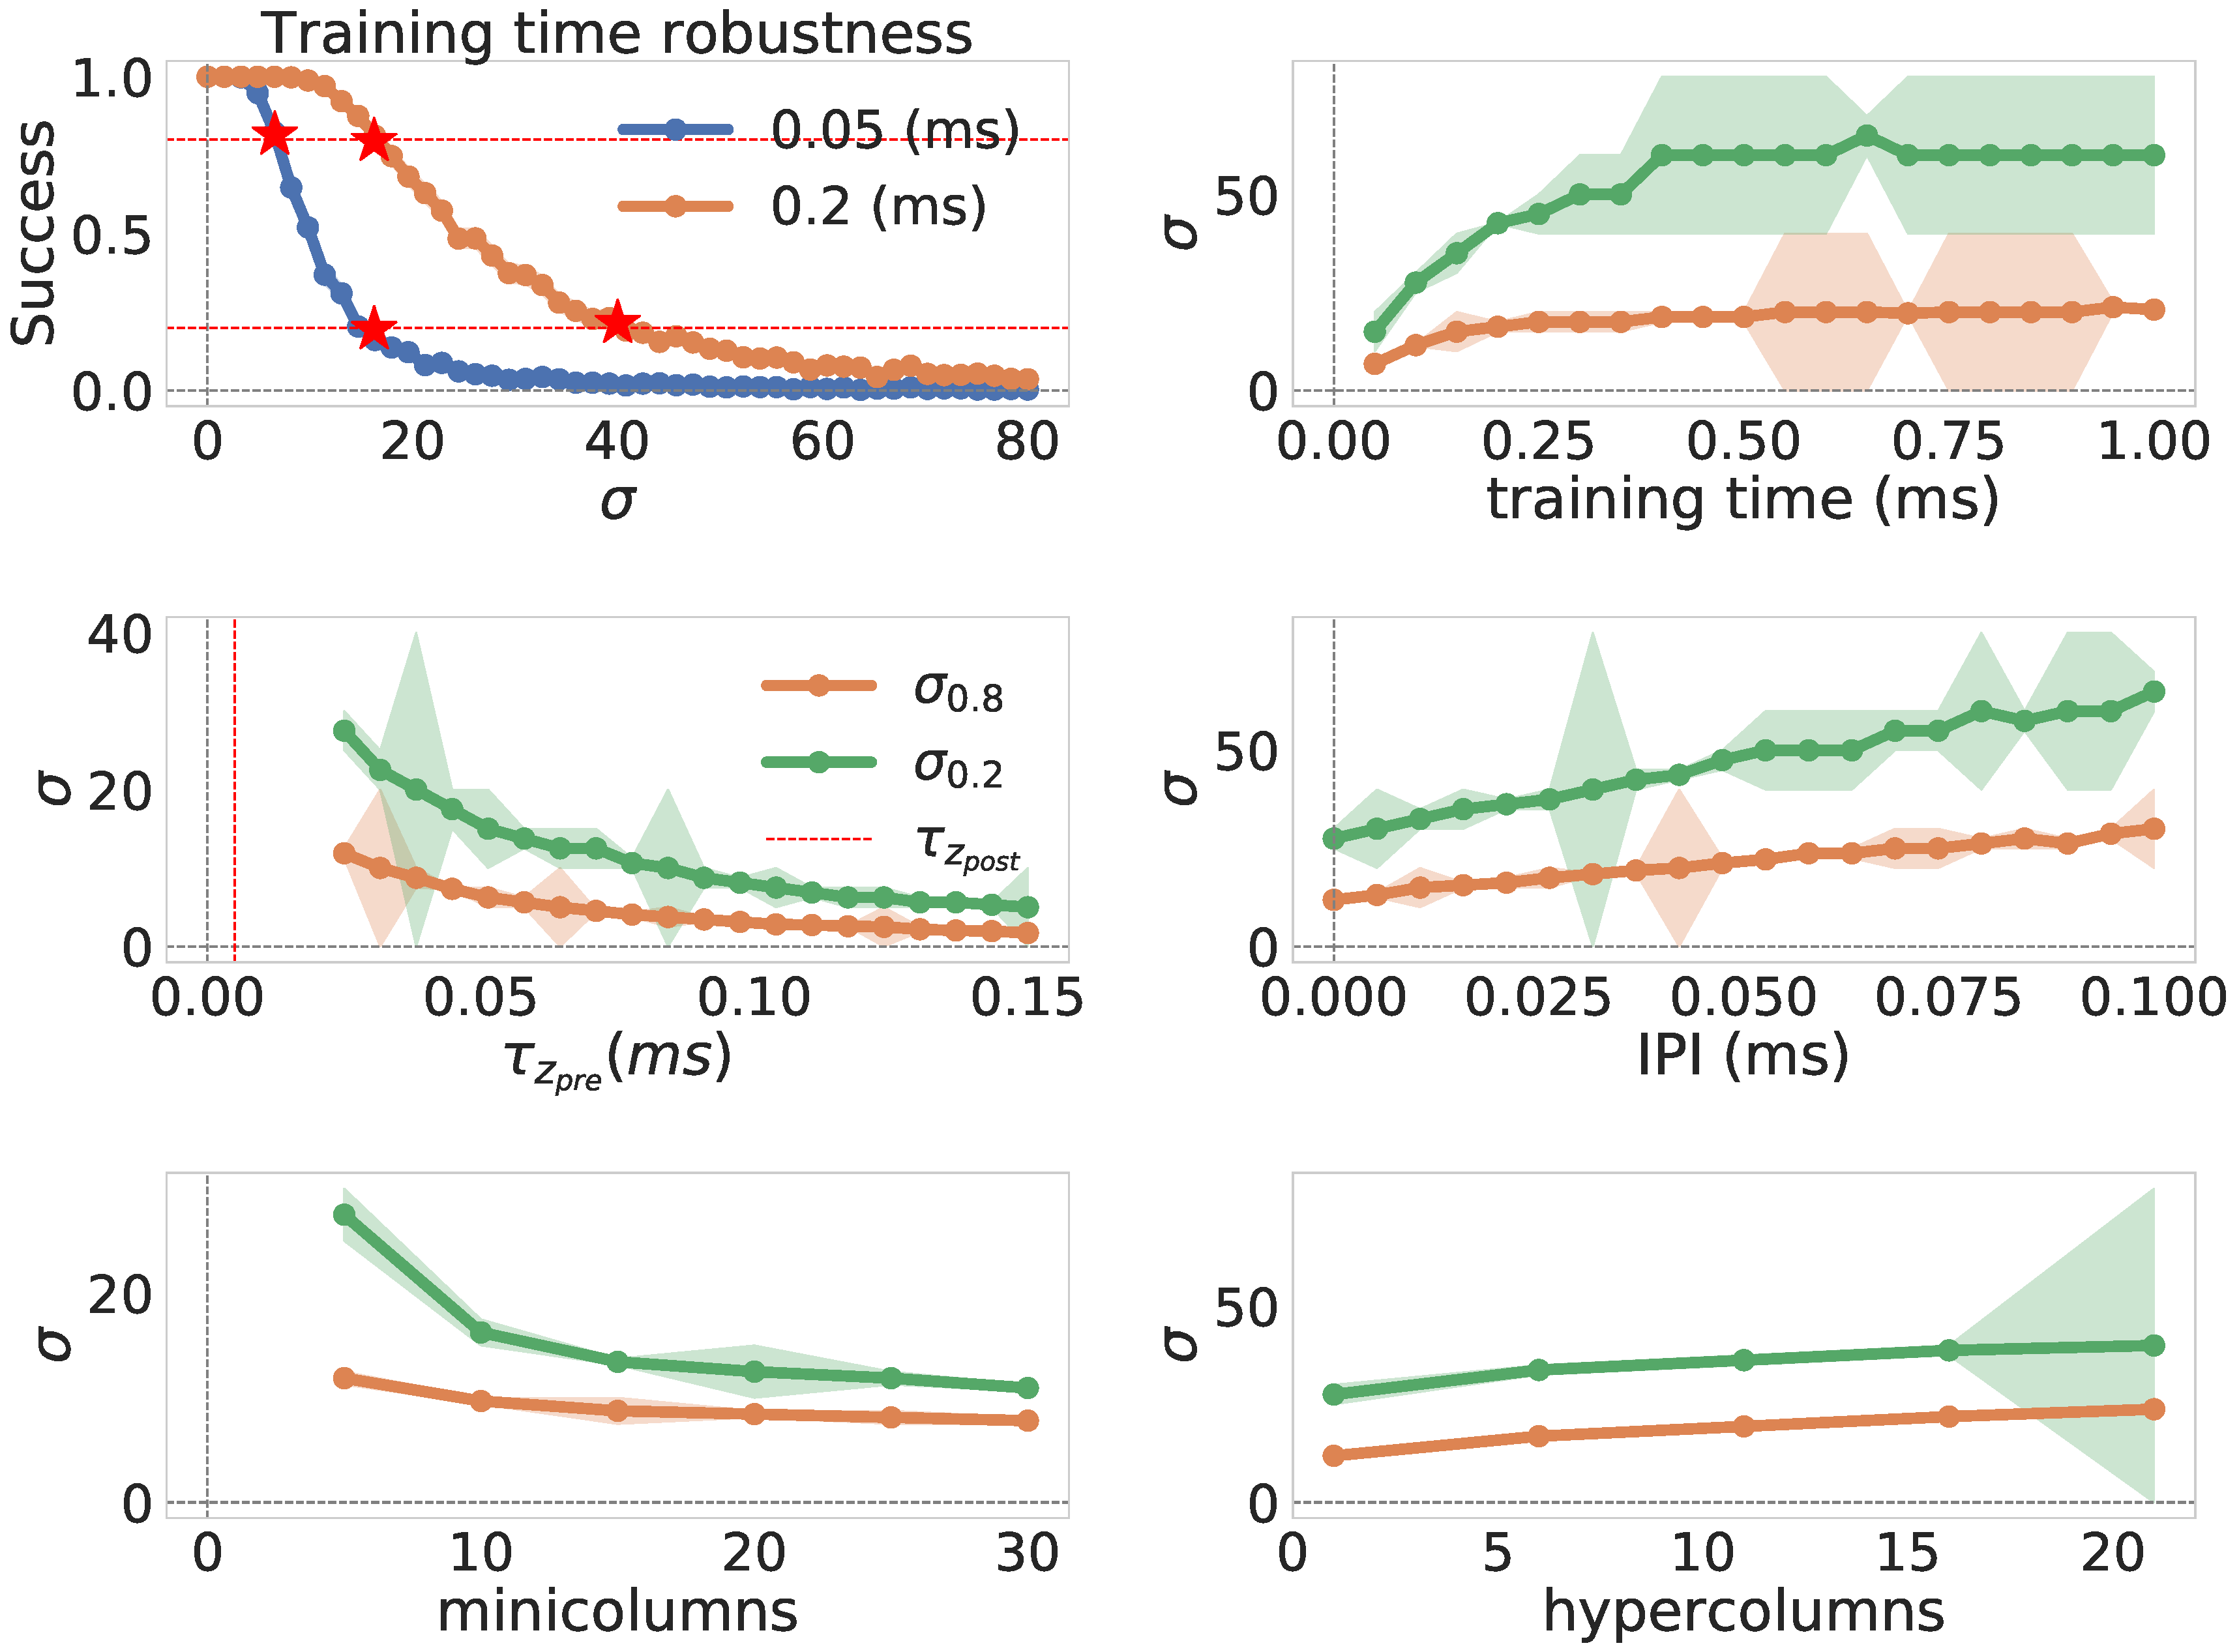
\includegraphics[scale=0.20]{noise_robustness_appendix.pdf}
\caption{$\sigma_{80}$ and $\sigma_{20}$ characterization}
\label{fig:appendix_noise_sensitivity}
\end{figure}


\bibliographystyle{apalike}
\bibliography{references.bib}

\end{document}